\documentclass[lang=cn,10pt,newtx]{elegantbook}
\usepackage{tikz}
\usepackage{tikz-imagelabels}
\usepackage{float}
\allowdisplaybreaks[4]
\newtheorem{Thm}{\hspace{2em}定理}[section]
\newcommand{\supp}{\text{supp}}
\newcommand{\dif}{\mathrm{d}}
\newcommand{\avg}[1]{\left\langle #1 \right\rangle}
\newcommand{\difFrac}[2]{\frac{\dif #1}{\dif #2}}
\newcommand{\pdfFrac}[2]{\frac{\partial #1}{\partial #2}}
\newcommand{\OFL}{\mathrm{OFL}}
\newcommand{\UFL}{\mathrm{UFL}}
\newcommand{\fl}{\mathrm{fl}}
\newcommand{\op}{\odot}
\newcommand{\cp}{\cdot}
\newcommand{\Eabs}{E_{\mathrm{abs}}}
\newcommand{\Erel}{E_{\mathrm{rel}}}
\newcommand{\DR}{\mathcal{D}_{\widetilde{LN}}^{n}}
\newcommand{\add}[2]{\sum_{#1=1}^{#2}}
\newcommand{\innerprod}[2]{\left<#1,#2\right>}
\newcommand{\norm}[1]{\|#1\|}
\newcommand\tbbint{{-\mkern -16mu\int}}
\newcommand\tbint{{\mathchar '26\mkern -14mu\int}}
\newcommand\dbbint{{-\mkern -19mu\int}}
\newcommand\dbint{{\mathchar '26\mkern -18mu\int}}
\newcommand\bint{
{\mathchoice{\dbint}{\tbint}{\tbint}{\tbint}}
}
\newcommand\bbint{
{\mathchoice{\dbbint}{\tbbint}{\tbbint}{\tbbint}}
}
\title{Note For Finite Element Methods}
\subtitle{Zhejiang University}

\author{Shuang Hu}
\institute{Zhejiang University}
\date{Sept 14, 2022}
\version{1.0}
\bioinfo{简介}{2022秋冬学季“有限元方法”课程笔记}

\setcounter{tocdepth}{3}

\logo{logo-blue.png}
\cover{cover.jpg}

% 本文档命令
\usepackage{array}
\newcommand{\ccr}[1]{\makecell{{\color{#1}\rule{1cm}{1cm}}}}

% 修改标题页的橙色带
\definecolor{customcolor}{RGB}{32,178,170}
\colorlet{coverlinecolor}{customcolor}
\usepackage{cprotect}

\addbibresource[location=local]{reference.bib} % 参考文献,不要删除

\begin{document}

\maketitle
\frontmatter

\tableofcontents

\mainmatter

\chapter{一维有限元方法}
\section{为什么需要有限元方法?}
此前在《微分方程数值解》课程中,我们已经学习了有限差分法和有限体积法。这两种方法有不少优点:首先,比较直观,只要知道如何利用差分近似导数即可得到对应的差分公式;其次,在一些情形下,有限差分和有限体积方法可以实现较高的计算精度。

但是,这两种算法有一些明显的缺陷。
\begin{itemize}
  \item 算法稳定性的分析比较复杂。
  \item 处理不规则区域的问题时较为麻烦,需要多次利用插值近似。
  \item 只是求解离散格点的近似点值/离散网格的近似积分平均值,未能给出函数整体的近似。
\end{itemize}

为此,基于函数逼近论的\textbf{有限元方法}被提出。该算法能弥补有限差分法的一些明显缺陷,目前是最主流的数值算法之一。
\section{从一维边值问题说起}
考虑如下例子:
\begin{equation}
  \label{eq:ode1}
  \left\{
    \begin{aligned}
    -u''+u&=f(x),x\in(0,1)\\
    u(0)=u(1)&=0.
    \end{aligned}
  \right.
\end{equation}
类似于“偏微分方程”课程中对弱解的讨论方式,在\eqref{eq:ode1}两边同时乘某个函数$v$并在$[0,1]$上积分,得到如下形式:
\begin{equation}
  \label{eq:bianfen}
  \int_{0}^{1}(-u''+u)v\dif x=\int_{0}^{1}fv\dif x.
\end{equation}
定义函数空间$V$如下:
\begin{equation}
  \label{eq:sobolev1-1}
  V:=\left\{v\left.\right|v(0)=v(1)=0,\int_{0}^{1}((v')^{2}+v^{2})\dif x<\infty\right\}.
\end{equation}
如果函数$v\in V$, 利用分部积分法,\eqref{eq:ode1}可以转化为以下问题:
\begin{example}
  \label{ex:equiv1}
  记$a(u,v)=\int_{0}^{1}(u'v'+uv)\dif x$, $h(v)=\int_{0}^{1}fv\dif x$, $v\in V$.求$u\in V$,使得$a(u,v)=h(v)$ $\forall v\in V$.
\end{example}
下面的定理说明了该问题可以转化为一个优化问题:
\begin{theorem}{}{}
  \label{thm:bianfen}
  记泛函$J(v):=\frac{1}{2}a(v,v)-h(v)$,问题\ref{ex:equiv1}与最小化$J(v)$的优化问题等价。即:如果$a(u,v)=h(v)\forall v\in V$, 那么$J(u)\le J(v)\forall v\in V$。
\end{theorem}
\begin{proof}
  $\Rightarrow$:
  \begin{equation}
    \label{eq:dif}
    \begin{aligned}
      J(v)-J(u)&=\frac{1}{2}a(v,v)-h(v)-\frac{1}{2}a(u,u)+h(u)\\
      &=\frac{1}{2}(a(v,v)-a(u,u)-2h(v-u))\\
      &=\frac{1}{2}(a(v,v)-a(u,u)-2a(u,v-u))\\
      &=\frac{1}{2}(a(v,v)+a(u,u)-2a(v,u))\\
      &=\frac{1}{2}(a(v-u,v-u))\ge0.
    \end{aligned}
  \end{equation}
  由\eqref{eq:dif}可得,如果$a(u,v)=h(v)$,那么$J(u)\le J(v)$.

  $\Leftarrow$: $\forall v\in V$, $t\in\mathbb{R}$,有$J(u+tv)\ge J(u)$。我们定义函数$g(t):=J(u+tv)$,根据上面的讨论可知:$g'(0)=0$。另一方面,计算$g(t)$的表达式,有:
  \begin{equation}
    \begin{aligned}
      \label{eq:gt}
      g(t)&=J(u+tv)\\
      &=\frac{1}{2}\int_{0}^{1}((u'+tv'
      )^{2}+(u+tv)^{2})\dif x-\int_{0}^{1}f(u+tv)\dif x\\
    \end{aligned}
  \end{equation}
  对\eqref{eq:gt}求一阶导数,可得:
  \begin{equation}
    \label{eq:dirg0}
    g'(0)=\int_{0}^{1}(u'v'+uv)\dif x-\int_{0}^{1}fv\dif x.
  \end{equation}
  根据$g$的一阶条件,可得$a(u,v)=h(v)$。又由于$v$的任意性,结论得证。
\end{proof}

如此,我们把一个解微分方程的问题,利用\ref{ex:equiv1}和\ref{thm:bianfen}转化为了一个变分问题。由于$V$是一个无穷维空间,我们不能期望利用算法给出这个变分问题的精确解,但我们可以考虑对空间$V$进行有限维近似,并在有限维空间上近似求解这个变分问题。

\section{有限元思想的导出}
接下来,根据上一节的思路,我们继续问题\eqref{eq:ode1}的近似求解。根据上面的分析,我们的数值算法需要解决两个问题:
\begin{itemize}
  \item 如何对函数空间$V$进行有限维近似?
  \item 在进行有限维近似之后,如何在有限维空间中对变分问题进行求解?
\end{itemize}
首先,我们考虑第二个问题。根据上面的讨论,近似求解变分问题有两种不同的思路,分别对应的是\textbf{Galerkin近似方法}和\textbf{Ritz近似方法}。
\subsection{Galerkin近似}
\textbf{假设已经给出有限维子空间}$V_{N}\le V$,Galerkin近似的目的是求解$u_{N}\in V_{N}$使得
\begin{equation}
  \label{eq:Galerkin}
  a(u_{N},v_{N})=h(v_{N})
\end{equation}
对所有$v_{N}\in V_{N}$都成立。

由于$V_{N}$是有限维的空间,我们可以找到这个空间中的一组基函数$\{\phi_{1},\cdots,\phi_{N}\}$,注意到$a(u,v)$是对称双线性函数,设$u_{N}=\alpha_{1}\phi_{1}(x)+\cdots+\alpha_{N}\phi_{N}(x)$,$v_{N}(x)=\phi_{i}(x)$,代入\eqref{eq:Galerkin},可得一个线性方程组:
\begin{equation}
  \label{eq:LinearSystem}
  \begin{bmatrix}
    a(\phi_{1},\phi_{1})&a(\phi_{1},\phi_{2})&\cdots&a(\phi_{1},\phi_{N})\\
    a(\phi_{2},\phi_{1})&a(\phi_{2},\phi_{2})&\cdots&a(\phi_{2},\phi_{N})\\
    \vdots&\vdots&\ddots&\vdots\\
    a(\phi_{N},\phi_{1})&a(\phi_{N},\phi_{2})&\cdots&a(\phi_{N},\phi_{N})\\
  \end{bmatrix}
  \begin{bmatrix}
    \alpha_{1}\\
    \alpha_{2}\\
    \vdots\\
    \alpha_{N}\\
  \end{bmatrix}
  =\begin{bmatrix}
    h(\phi_{1})\\
    h(\phi_{2})\\
    \vdots\\
    h(\phi_{N})\\
  \end{bmatrix}
\end{equation}
解这个线性方程组,得到系数向量,即可给出该方程的近似解。

\subsection{Ritz方法}
同样,假设有限维子空间$V_{N}\le V$已经给出,\textbf{Ritz方法}的思路是求解有关$J(u)$的优化问题,即:求$u_{N}\in V_{N}$,使得
\begin{equation}
J(u_{N})\le J(v)\forall v\in V_{N}.
\end{equation}
这里$J(v):=\frac{1}{2}a(v,v)-h(v)$。

给出这个问题之后,我们在有限维空间中,利用最优化算法求解该问题。

这两个思路都是建立在有限维子空间$V_{N}$已经给出的前提下的。但这个有限维空间如何构造?

一个很容易想到的思路是利用$v(0)=v(1)$这一性质,构造三角函数系作为基底。这种选取思路对于问题\eqref{eq:ode1}而言当然是极好的,三角函数系的正交性也使得\eqref{eq:LinearSystem}中的系数矩阵变得相当简单易求解。但这个方案的可扩展性并不强,如果扩展到二维平面上,乃至更高维度的椭圆偏微分方程,就很难找到像这样全局定义的基函数。如果问题区域非规则或是存在不同方程的耦合,则更是如此。

\textbf{有限元方法}由此引出。
\section{有限元方法}
在上面两种思路的基础上,我们需要一个方便推广的构建有限维子空间的方法。

多项式函数空间是最容易表示的函数空间,因此这是我们的首选。但全局定义的多项式很难保证其符合边界条件。于是,借助样条插值的思想,我们转为考虑分段多项式空间。

\subsection{线性有限元空间}
我们先针对问题\eqref{eq:ode1},考虑最简单的近似形式--分段线性近似。在这种情形下,有限维子空间$V_{h}$由$(0,1)$上的分段线性函数表示。
\begin{definition}{线性有限元空间}
  \label{LinearFE}
  线性有限元空间的定义为:
  \begin{equation}
    \label{eq:linearFE}
    V_{h}:=\{v_{h}\in C(0,1):v_{h}(0)=v_{h}(1)=0,v_{h}|_{[x_{i},x_{i+1}]}\in\mathbb{P}_{1}\}.
  \end{equation}
  其中$\{x_{i}\}_{i=0}^{n}$为$[0,1]$上给定的互异节点,$x_{0}=0$,$x_{n}=1$。
\end{definition}
首先需要讨论的是,空间$V_{h}$的维数和基底。空间\eqref{eq:linearFE}的形式很容易联想到数值分析课程中学习过的\textbf{B-样条空间}。特别地,一维B-样条基函数为所谓的“hat-function”,定义如下:
\begin{equation}
  \label{eq:hatfunc}
  \phi_{i}(x)=\left\{
    \begin{aligned}
      &\frac{x-x_{i-1}}{x_{i}-x_{i-1}},x_{i-1}\le x\le x_{i}\\
      &\frac{x_{i+1}-x}{x_{i+1}-x_{i}},x_{i}\le x\le x_{i+1}\\
      & 0,otherwise\\
    \end{aligned}
  \right.
\end{equation}
\begin{figure}[H]
  \centering
  \caption{hat函数的示意图}
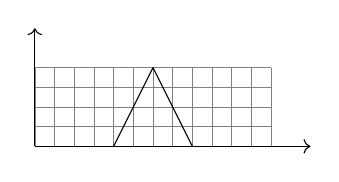
\begin{tikzpicture}
  \draw[step=.25cm,gray,very thin] (0,0) grid (3,1); 
  \draw [->](0,0) -- (3.5,0); 
  \draw [->](0,0) -- (0,1.5); 
  \draw (1,0) -- (1.5,1);
  \draw (1.5,1) -- (2,0);
\end{tikzpicture}
\end{figure}
容易验证,如此定义的$(\phi_{1},\cdots,\phi_{n-1})$构成了空间$V_{h}$的一组基。从而可得$\dim(V_{h})=n-1$。
\subsection{刚度矩阵与负载}
此处我们采用Galerkin近似的思路,下面我们需要讨论的是方程组\eqref{eq:LinearSystem}的导出与求解。

\begin{definition}{刚度矩阵}
  线性有限元空间\ref{LinearFE}的刚度矩阵定义为:
  \begin{equation}
    \label{eq:stablemat}
    A=(a(\phi_{i},\phi_{j}))_{i,j=1}^{n-1}.
  \end{equation}
  其中$\phi_{i}$为\eqref{eq:hatfunc}中定义的基函数。
\end{definition}

\begin{definition}{负载}
  方程\eqref{eq:ode1}关于线性有限元空间\ref{LinearFE}的负载向量定义为:
  \begin{equation}
    \label{eq:overload}
    \mathbf{b}:=\left(\int_{0}^{1}f(x)\phi_{i}(x)\dif x\right)_{i=1}^{n-1}.
  \end{equation}
\end{definition}

下面讨论\eqref{eq:ode1}负载的计算。由于我们是用一次样条多项式近似真实解的,在选取数值积分公式的时候只需要使用一阶代数精度的公式即可不损失计算精度。因此此处采用复化梯形公式进行负载的近似计算。

记$h_{i}=x_{i}-x_{i-1}$,负载的近似计算公式如下:
\begin{equation}
  b_{i}=\int_{0}^{1}f(x)\phi_{i}(x)\dif x=\int_{x_{i-1}}^{x_{i+1}}f(x)\phi_{i}(x)\approx \frac{1}{2}(h_{i}+h_{i+1})f(x_{i}).
\end{equation}

对于刚度矩阵的计算,虽然基函数$\phi_{i}$在整个区间$(0,1)$上并不可导,但不可导点为零测集,不会对积分的计算产生影响。将基函数$\phi_{i}$的表达式代入刚度矩阵,计算得:
\begin{equation}
  \label{eq:stablematval}
  \left\{
    \begin{aligned}
      a_{ij}&=0,|i-j|>1\\
      a_{ii}&=\frac{1}{h_{i}}+\frac{1}{h_{i+1}}+\frac{1}{3}(h_{i}+h_{i+1})\\
      a_{i-1,i}&=-\frac{1}{h_{i}}+\frac{1}{6}h_{i}\\
      a_{i,i+1}&=-\frac{1}{h_{i+1}}+\frac{1}{6}h_{i+1}\\
    \end{aligned}
  \right.
\end{equation}
由\eqref{eq:stablematval}可知,刚度矩阵是一个三对角矩阵,因此如果采用传统的矩阵存储方式和求解方式可能会造成计算资源的浪费。下面给出一种采用“局部矩阵”的形式存储\eqref{eq:stablematval}的技巧。

记负载矩阵$A=\sum_{k=1}^{n}A^{(k)}$,其中$A^{(k)}:=(a_{ij}^{(k)})$,$a_{ij}^{(k)}:=\int_{x_{k-1}}^{x_{k}}[\phi_{i}'(x)\phi_{j}'(x)+\phi_{i}(x)\phi_{j}(x)]\dif x$,由定义可得,$a_{ij}^{(k)}$只在$i,j\in\{k-1,k\}$时取非零值。所以每个$A^{(k)}$都可以存储为一个$2\times 2$的矩阵,而整体的负载矩阵$A$可以视为把所有的$A^{(k)}$“装配”起来的结果。在求解最终的线性方程组的时候,由于矩阵$A$是一个三对角对称正定矩阵,我们可以采用一系列数值代数算法加速方程组的求解。
\section{误差分析}
在本节中我们针对求解\eqref{eq:ode1}的线性有限元近似算法进行误差分析。在叙述之前,为方便起见,先给出两个记号。

\begin{remark}
  $\norm{f}_{0}$:表示$L^{2}$范数, $\norm{f}_{0}:=\sqrt{\int_{0}^{1}f^{2}\dif x}$。$\norm{f}_{1}$:表示$W^{1,2}$范数,$\norm{f}_{1}:=\sqrt{\int_{0}^{1}((f')^{2}+f^{2})\dif x}$。
\end{remark}

回顾一下有限元逼近问题的提法:
\begin{example}
  \label{prob:FE problem}
记泛函$a(u,v)=\int_{0}^{1}(uv+u'v')\dif x$, $h(v)=\int_{0}^{1}fv\dif x$, $V=\{v(x):v(0)=v(1)=0,\int_{0}^{1}((v')^{2}+v^2)\dif x<\infty\}$, 原问题是求解$u\in V$使得$a(u,v)=h(v)\forall v\in V$, 而在线性有限元空间上的逼近问题则是,在线性有限元空间$V_{h}\le V$上求解$u_{h}\in V$使得$a(u_{h},v_{h})=h(v_{h})\forall v_{h}\in V_{h}$。
\end{example}

在进行讨论前,首先给出一个重要的引理。该引理保证了在$W^{1,2}$范数的意义下,$u_{h}\in V_{h}$是$u\in V$在子空间$V_{h}$下的最优逼近。
\begin{lemma}{Cea引理}
  \label{lem:cea}
  设$u$和$u_{h}$是\ref{prob:FE problem}的解,则有:
  \begin{equation}
    \label{eq:cea}
    \norm{u-u_{h}}_{1}\le\inf_{v_{h}\in V_{h}}\norm{u-v_{h}}_{1}.
  \end{equation}
\end{lemma}
\begin{proof}
  由于$u$满足:$\forall v\in V, a(u,v)=h(v)\Rightarrow\forall v_{h}\in V_{h},a(u,v_{h})=h(v_{h})$。又有:$u_{h}$满足$a(u_{h},v_{h})=h(v_{h})\forall v_{h}\in V_{h}$,两式相减,得:
  \begin{equation}
    \label{eq:orthogonal}
    a(u-u_{h},v_{h})=0\,\forall v\in V_{h}.
  \end{equation}
  \eqref{eq:orthogonal}表示了向量$u-u_{h}$和空间$V_{h}$的正交性。下面讨论$\norm{u-u_{h}}_{1}^{2}$的估计。
  \begin{equation}
    \label{eq:estimateError}
    \begin{aligned}
    \norm{u-u_{h}}_{1}^{2}&=a(u-u_{h},u-u_{h})\\
    &=a(u-u_{h},u-v_{h})\\
    &=\int_{0}^{1}((u'-u_{h}')(u'-v_{h}')+(u-u_{h})(u-v_{h}))\dif x\\
    &\le\left(\int_{0}^{1}(u'-u_{h}')^{2}\dif x\right)^{\frac{1}{2}}\left(\int_{0}^{1}(u'-v_{h}')^{2}\right)^{\frac{1}{2}}+\left(\int_{0}^{1}(u-u_{h})^{2}\right)^{\frac{1}{2}}\left(\int_{0}^{1}(u-v_{h})^2\right)^{\frac{1}{2}}\\
    &\le\left\{\int_{0}^{1}\left((u'-u_{h}')^{2}+(u-u_{h})^{2}\right)\dif x\right\}^{\frac{1}{2}}\left\{\int_{0}^{1}\left((u'-v_{h}')^2+(u-v_{h})^{2}\right)\dif x\right\}^{\frac{1}{2}}\\
    &=\norm{u-u_{h}}_{1}\norm{u-v_{h}}_{1}\Rightarrow\norm{u-u_{h}}_{1}\le\norm{u-v_{h}}_{1}.\\
    \end{aligned}
  \end{equation}
\end{proof}
该引理在$\norm{\cdot}$的意义下,把有限元解的误差转化为计算解函数的插值误差(这个插值误差可以作为一个上界)。目前解函数用$u$表示,假设$u$在节点$\{x_{i}\}_{i=0}^{n}$上的分段线性插值多项式记为$u_{I}$,考虑$\norm{u-u_{I}}_{1}$的估计。关于分段线性插值,我们有下面的误差估计公式:
\begin{theorem}
  \label{thm:interperror}
  \begin{equation}
    \left\{
      \begin{aligned}
        \max_{[0,1]}|u(x)-u_{I}(x)|&\le\frac{1}{8}h^2\max_{[0,1]}|u''(x)|\\
        \max_{[0,1]}|u'(x)-u_{I}'(x)|&\le h\max_{[0,1]}|u''(x)|\\
      \end{aligned}
    \right.
  \end{equation}
  其中$h=\max_{1\le i\le n}|x_{i}-x_{i-1}|$。
\end{theorem}
\begin{proof}
  见任何一本数值分析教材。
\end{proof}
根据\ref{thm:interperror}和\ref{lem:cea},可以针对$\norm{u-u_{h}}_{1}$进行估计。
\begin{equation}
  \label{eq:ceaestimate}
  \norm{u-u_{h}}_{1}^{2}\le\norm{u-u_{I}}_{1}^{2}=\int_{0}^{1}((u-u_{I})^{2}+(u'-u_{I}')^{2})\dif x\le(\frac{1}{64}h^{4}+h^{2})\max_{[0,1]}|u''(x)|^{2}.
\end{equation}
从而,我们导出了下面的估计定理:
\begin{theorem}
  \label{thm:estimatebyinftynorm}
  \begin{equation}
    \norm{u-u_{h}}_{1}\le 2h\max_{[0,1]}|u''|.
  \end{equation}
\end{theorem}
\ref{thm:estimatebyinftynorm}给出了利用无穷范数控制$\norm{\cdot}_{1}$的方法。但由于二阶求导可能会大幅度提升$u$的振幅,$\max_{[0,1]}|u''|$可能会大的令人难以接受,所以我们最好能找到更合理的范数估计。事实上,如果右端项取$u''$的$L^{2}-norm$,我们可以有下面的估计:
\begin{theorem}
  \label{thm:estimatebyL2}
  \begin{equation}
    \norm{u-u_{h}}_{1}\le Ch\norm{u''}_{0}\le Ch\norm{f}_{0}.
  \end{equation}
\end{theorem}
\begin{proof}
在介绍\ref{thm:estimatebyL2}的证明前,我们需要先给出一些命题。
\newpage
\begin{proposition}
  \label{prop:enermy}
  如果$w\in C^{2}$是下面的微分方程的解:
  \begin{equation}
    \label{eq:odeforw}
    \left\{
      \begin{aligned}
        &-w''+w=g(x),x\in(0,1),\\
        &w(0)=w(1)=0.\\
      \end{aligned}
    \right.
  \end{equation}
  则有
  \begin{equation}
    \label{eq:enermy-norm}
  \int_{0}^{1}(w'')^{2}\dif x\le\int_{0}^{1}g^{2}\dif x.
  \end{equation}
\end{proposition}
\begin{proof}
  在\eqref{eq:odeforw}的第$(1)$式左右两边同乘$w''$,并同时在区间$[0,1]$上积分: 
  \begin{equation}
    \begin{aligned}
      &\int_{0}^{1}(-w''+w)w''\dif x=\int_{0}^{1}g(x)w''(x)\dif x\\
      \Rightarrow&\int_{0}^{1}(w'')^{2}\dif x+\int_{0}^{1}(w')^{2}\dif x=-\int_{0}^{1}g(x)w''(x)\dif x\\
      \Rightarrow&\int_{0}^{1}(w'')^{2}\dif x\le\int_{0}^{1}g(-w'')\dif x\le \norm{g}_{0}\norm{w''}_{0}\\
      \Rightarrow&\norm{w''}_{0}\le\norm{g}_{0}\\
    \end{aligned}
  \end{equation}
\end{proof}
\begin{remark}
  该结论的证明思路正是偏微分方程理论中非常常见的“能量模估计”。
\end{remark}
\begin{proposition}
  \label{prop:Gxt}
  记
  \begin{equation}
    \label{eq:Gxt}
    G_{i}(x,t)=\left\{
      \begin{aligned}
        &(t-x_i)(x-x_{i+1}),x>t ,\\
        &(x-x_{i})(t-x_{i+1}),x\le t.\\
      \end{aligned}
    \right.
  \end{equation}
  那么在$[x_{i},x_{i+1}]$上,有下面这一等式成立:
  \begin{equation}
    (u(x)-u_{I}(x))(x_{i+1}-x_{i})=\int_{x_{i}}^{x_{i+1}}G_{i}(x,t)u''(t)\dif t.
  \end{equation}
\end{proposition}
\begin{proof}
  记符号$h_{i}:=x_{i+1}-x_{i}$,计算右端项的积分,有:
  \begin{equation}
    \begin{aligned}
      &\int_{x_{i}}^{x_{i+1}}G_{i}(x,t)u''(t)\dif t\\
      =&(x-x_{i+1})\int_{x_{i}}^{x}(t-x_{i})u''(t)\dif t+(x-x_{i})\int_{x}^{x_{i+1}}u''(t)(t-x_{i+1})\dif t\\
      =&(x-x_{i+1})\left[\int_{x_{i}}^{x}(t-x_{i})\dif u'(t)\right]+(x-x_{i})\left[\int_{x}^{x_{i+1}}(t-x_{i})\dif u'(t)\right]\\
      =&(x-x_{i+1})\left[(x-x_{i})u'(x)-\int_{x_{i}}^{x}u'(t)\dif t\right]+(x-x_{i})\left[(x_{i+1}-x)u'(x)-\int_{x}^{x_{i+1}}u'(t)\dif t\right]\\
      =&h_{i}u(x)+(x-x_{i+1})u(x_{i})-(x-x_{i})u(x_{i+1})\\
      =&h_{i}(u(x)-u_{I}(x)).\\
    \end{aligned}
  \end{equation}
  \end{proof}
  下面利用\ref{prop:enermy}和\ref{prop:Gxt}证明定理\ref{thm:estimatebyL2}。首先讨论$\norm{u-u_{1}}_{0}$的估计。由\ref{prop:Gxt},我们有:
  \begin{equation}
    \label{eq:norm0-estimate}
    \begin{aligned}
      \int_{0}^{1}[u(x)-u_{I}(x)]^{2}\dif x&=\sum_{i=0}^{n-1}\int_{x_{i}}^{x_{i+1}}[u(x)-u_{I}(x)]^{2}\dif x\\
      &=\sum_{i=0}^{n-1}\int_{x_{i}}^{x_{i+1}}\left[\frac{1}{x_{i+1}-x_{i}}\int_{x_{i}}^{x_{i+1}}G_{i}(x,t)u''(t)\dif t\right]^{2}\dif x.\\
      &\le\sum_{i=0}^{n-1}(x_{i+1}-x_{i})\left[\frac{1}{x_{i+1}-x_{i}}\int_{x_{i}}^{x_{i+1}}(t-x_{i})(x_{i+1}-t)|u''(t)|\dif t\right]^{2}\\
      &\le\sum_{i=0}^{n-1}(x_{i+1}-x_{i})\left[\frac{x_{i+1}-x_{i}}{4}\int_{x_{i}}^{x_{i+1}}|u''(t)|\dif t\right]^{2}\\
      &\le\sum_{i=0}^{n-1}\frac{(x_{i+1}-x_{i})^{3}}{16}\left[\int_{x_{i}}^{x_{i+1}}|u''(t)|\dif t\right]^{2}\allowdisplaybreaks[4]\\
      &\le\sum_{i=0}^{n-1}\frac{(x_{i+1}-x_{i})^{4}}{16}\int_{x_{i}}^{x_{i+1}}|u''(t)|^{2}\dif t\\
      &\le\frac{h^4}{16}\int_{0}^{1}|u''(t)|^{2}\dif t.
    \end{aligned}
  \end{equation}
  \eqref{eq:norm0-estimate}中,第三行和第四行的不等式都源于对函数$G_{i}(x,t)$的估计,第六行的不等式则源于柯西不等式。
  
  由\ref{prop:Gxt}可知,在$[x_{i},x_{i+1}]$上,我们有:
  \begin{equation}
    \label{eq:dir}
    \begin{aligned}
    |u'(x)-u_{I}'(x)|&=\left|\frac{1}{x_{i+1}-x_{i}}\left[\int_{x_{i}}^{x}\frac{(t-x_{i})u''(t)}{x_{i+1}-x_{i}}\dif t+\int_{x}^{x_{i+1}}\frac{(t-x_{i+1})u''(t)}{x_{i+1}-x_{i}}\dif t\right]\right|\\
    &\le C(x_{i+1}-x_{i})^{\frac{1}{2}}\left(\int_{x_{i}}^{x_{i+1}}|u''(t)|^{2}\dif t\right)^{\frac{1}{2}}.
    \end{aligned}
  \end{equation}
  \eqref{eq:dir}中,$C$为常数,该不等式由柯西不等式导出。借助该式,我们有:
  \begin{equation}
    \label{eq:direstimate}
    \begin{aligned}
      \int_{0}^{1}|u'(x)-u_{I}'(x)|^{2}\dif x&=\sum_{i=0}^{n-1}\int_{x_{i}}^{x_{i+1}}[u'(x)-u_{I}'(x)]^{2}\dif x\\
      &\le\sum_{i=0}^{n-1}C^{2}(x_{i+1}-x_{i})^{2}\int_{x_{i}}^{x_{i+1}}|u''(t)|^{2}\dif t\\
      &\le C^{2}h^{2}\int_{0}^{1}|u''(t)|^{2}\dif t.
    \end{aligned}
  \end{equation}
  联立\eqref{eq:norm0-estimate}和\eqref{eq:direstimate},结合引理\ref{lem:cea}和命题\ref{prop:enermy},定理\ref{thm:estimatebyL2}得证。
\end{proof}
\begin{remark}
  对\ref{thm:estimatebyL2},可以用Fourier分析给出一个更优的估计。
\end{remark}
\begin{exercise}
  补充\eqref{eq:direstimate}的证明细节,并给出常数$C$的值。
\end{exercise}
利用定理\ref{thm:estimatebyL2},对于$\norm{u-u_{h}}_{0}$,我们可以给出更精细的估计:
\begin{theorem}{Aubin-Nitsche技巧}
  \begin{equation}
    \label{eq:AubinNitsche}
    \norm{u-u_{h}}_{0}\le Ch^{2}\norm{u''}_{0}.
  \end{equation}
\end{theorem}
\begin{proof}
  考虑辅助问题:
  \begin{equation}
    \label{eq:auxiliaryProb}
    \left\{
    \begin{aligned}
        -z''+z&=u-u_{h},\\
        z(0)=z(1)&=0.\\
    \end{aligned}
    \right.
  \end{equation}
  其变分形式为:
  \begin{equation}
    a(z,v)=(u-u_{h},v)_{L^{2}},\,\forall v\in V.
  \end{equation}
  从而:
  \begin{equation}
    \begin{aligned}
      \norm{u-u_{h}}_{0}&=a(z,u-u_{h})\\
      &=a(z-\omega_{h},u-u_{h})\,\forall\omega_{h}\in V_{h}\\
    \end{aligned}
  \end{equation}
  取$\omega_{h}$为函数$z$的分段线性插值$z_{I}$,那么:
  \begin{equation}
    a(z-z_{I},u-u_{h})\le C\norm{z-z_{I}}_{1}\norm{u-u_{h}}_{1}\le Ch^{2}\norm{z''}_{0}\norm{f}_{0}.
  \end{equation}
  由 \eqref{eq:enermy-norm},$\norm{z''}_{0}\le C\norm{u-u_{h}}_{0}$,结论得证。
\end{proof}
\section{一阶非齐次BVP}
接下来我们把研究对象改为一般的非齐次两点边值问题。事实上,虽然方程看似复杂了些,但处理方法和之前基本一致。

考虑下面的例子:
\begin{equation}
  \label{eq:unhomobvp}
  \left\{
    \begin{aligned}
      &-(k(x)u')'+q(x)u=f(x),\;x\in(0,1),\\
      &u(0)=\alpha,\; u(1)=\beta.
    \end{aligned}
  \right.
\end{equation}
其中$k(x)\in C^{1}$, $k(x)\ge k_{0}>0$, $q(x)\ge 0$.

和齐次问题同样的道理,先考虑该问题的变分形式。在\eqref{eq:unhomobvp}两端同乘函数$v$并在$[0,1]$上积分,有:
\begin{equation}
  \label{eq:bianfen2}
  \begin{aligned}
  &\int_{0}^{1}[-(k(x)u')'v(x)+q(x)u(x)v(x)]\dif x=\int_{0}^{1}f(x)v(x)\dif x\\
  \Rightarrow &\int_{0}^{1}quv\dif x-\int_{0}^{1}v(x)\dif(k(x)u')=\int_{0}^{1}f(x)v(x)\dif x\\
  \Rightarrow &\int_{0}^{1}(quv+ku'v')\dif x+v(0)k(0)u'(0)-v(1)k(1)u'(1)=\int_{0}^{1}f(x)v(x)\dif x.\\
  \end{aligned}
\end{equation}
要保证\eqref{eq:bianfen2}有意义,同样需要确保$u,v\in V:=W^{1,2}$。在此基础上,如果$v(0)=v(1)=1$,令
$a(u,v):=\int_{0}^{1}(ku'v'+quv)\dif x$,$h(v):=\int_{0}^{1}fv\dif x$,则有:
\begin{equation}
  \label{eq:unhomobianfen}
  a(u,v)=h(v)\;\forall v\in V,\; v(0)=v(1)=0.
\end{equation}
其中$u\in W:=\{v:\int_{0}^{1}((v')^{2}+v^2)\dif x<\infty, v(0)=\alpha, v(1)=\beta\}.$

同样地,该问题也有与之相对应的极小化问题:
\begin{example}
  \label{ex:optimal2}
  求$u\in W$ s.t. $J(u)\le J(v)\forall v\in W$, 此处$J(v):=\frac{1}{2}a(v,v)-f(v)$。
\end{example}

下一步则是构造对应的线性有限元空间。注意到,对于非齐次边值问题,函数集合$W$并不构成线性空间,所以我们构建的“线性有限元空间”实际上是一个由分段线性函数构成的子集。但与此同时,这个子集可以写成陪集(coset)的形式,所以我们依旧可以利用基底的线性组合来表示这个函数集合。

取$[0,1]$区间的分划$0=x_{0}<x_{1}<\cdots<x_{n-1}<x_{n}=1$,由于$u(0)=\alpha,u(1)=\beta$,记函数集合$W_{h}:=\{w\in C(0,1):w|_{[x_{i},x_{i+1}]}\in\mathbb{P}_{1},w(0)=\alpha,w(1)=\beta\}$,那么我们必定有$u\in W_{h}$。$V_{h}$的定义同\ref{eq:linearFE},设分段线性函数$g(x)$满足:
\begin{equation}
  \label{eq:segmentlinearcondition}
  g(0)=\alpha,g(1)=\beta,\forall i\in[1,n-1],g(x_{i})=0.
\end{equation}
那么我们有$W_{h}=g+V_{h}$。

最后考虑有限元近似求解。此处$\phi_{i}$的定义沿用\eqref{eq:hatfunc}的表达式,记$u_{h}(x):=g(x)+\sum_{i=1}^{n-1}\alpha_{i}\phi_{i}(x)$,$v_{i}(x):=\phi_{i}(x)$,代入\eqref{eq:unhomobianfen},得:
\begin{equation}
  \label{eq:FEfenliang}
  a(g,\phi_{i})+\sum_{j=1}^{n-1}\alpha_{j}a(\phi_{j},\phi_{i})=h(\phi_{i}).
\end{equation}
由$a(\cdot,\cdot)$的对称性,我们把\eqref{eq:FEfenliang}转化为矩阵形式$(Ax=b)$。其中刚度矩阵$A:=a(\phi_{i},\phi_{j})_{i,j=1}^{n-1}$,负载$b:=(h(\phi_{i})-a(g,\phi_{i}))^{t}$。可以证明,刚度矩阵仍旧为对称正定三对角矩阵。但刚度矩阵和负载向量的计算则需要通过数值积分完成。当然,在编程计算刚度矩阵时,利用装配技巧同样能节省存储空间并增加程序的可读性。

与齐次方程同样,非齐次方程变分问题的有限元解也有与之相对应的Cea引理和各种范数估计,且证明方法近乎雷同,故此处省略不表,留作习题。

\begin{remark}
  \eqref{eq:unhomobvp}中$q(x)\ge 0$的条件似乎应当改为$q(x)\ge q_{0}>0$,否则Cea引理的证明会出问题。举个例子,如果$q(x)\equiv 0$,引出的就不再是对$\norm{u-u_{h}}_{1}$的估计,而是$\norm{u'-u_{h}'}_{0}$的估计。
\end{remark}
\section{其他边值问题}
\subsection{Neumann边值问题}
问题描述:
\begin{equation}
  \label{eq:Neumann}
  \left\{
    \begin{aligned}
    &-(ku')'+qu=f\\
    &-k(0)u'(0)=\gamma_{1},k(1)u'(1)=\gamma_{2}\\
    \end{aligned}
  \right.
\end{equation}

变分形式:
\begin{equation}
  \int_{0}^{1}(ku'v'+quv)\dif x=\int_{0}^{1}fv\dif x+\gamma_{2}v(1)+\gamma_{1}v(0).
\end{equation}
\subsection{Robin边值问题}
问题描述:
\begin{equation}
  \label{eq:Robin}
  \left\{
    \begin{aligned}
    &-(ku')'+qu=f\\
    &-k(0)u'(0)=-\beta_{1}u(0)+\gamma_{1},k(1)u'(1)=-\beta_{2}u(1)+\gamma_{2}\\
    \end{aligned}
  \right.
\end{equation}

变分形式:
\begin{equation}
  \int_{0}^{1}(ku'v'+quv)\dif x=\int_{0}^{1}fv\dif x+\gamma_{1}v(0)+\gamma_{2}v(1)-\beta_{1}u(0)v(0)-\beta_{2}u(1)v(1).
\end{equation}

\section{本章总结}
有限元的基本逻辑:
\begin{itemize}
  \item 两边相乘试验函数,同时积分。
  \item 给出变分形式。
  \item 构造函数空间的有限维子空间。
  \item 在有限维子空间上求解变分形式。
  \item 误差估计。
\end{itemize}
由于有限元方法的输出并非解函数在某些点上的取值或者控制体上的积分平均值,而是整体函数,其误差范数定义和有限差/有限体方法有一些区别。本章中常用的范数是$L^{2}$范数和$W^{1,2}$范数。同样,由于有限元方法是在函数空间中求解优化问题或者线性方程,函数逼近论在有限元方法的研究中居于重要地位。

\chapter{变分原理}
上一章中,我们用一个具体的例子说明了有限元的大体思路和操作步骤。本章则会着眼于变分问题的提法,给出一般情形下的变分问题(以及其等价形式),并证明其解的存在唯一性。最后则是给出几个具体的算例以及它们各自的变分形式。
\section{变分问题以及等价形式}
在上一章定理\ref{thm:bianfen}中,我们针对一个特殊问题,提出了两种变分问题,并证明了这两种问题的等价性。本节中,我们将着眼于更一般的问题,并对一般的问题尝试说明两者的等价性,以及其解的存在唯一性。在此之前,先要做一些概念和定理上的准备。
\subsection{预备知识}
首先,我们讨论双线性函数。
\begin{definition}{双线性函数}
  一个\textbf{双线性函数}$a(\cdot,\cdot):V\times V\rightarrow\mathbb{R}$需要满足下面的条件:
  \begin{itemize}
    \item $a(k_{1}u+k_{2}v,w)=k_{1}a(u,w)+k_{2}a(v,w)$.
    \item $a(u,k_{1}v+k_{2}w)=k_{1}a(u,v)+k_{2}a(u,w)$.
  \end{itemize}
  对任意$u,v\in V$, $k_{1},k_{2}\in F$均成立。特别地,假设$V$是以$\norm{\cdot}$为范数的赋范线性空间,如果对任意$u,v\in V$,存在$M>0$使得:
  \begin{equation}
    \label{eq:bddbilinear}
    |a(u,v)|\le M\norm{u}\norm{v}
  \end{equation}
  总成立,那么我们称双线性型$a$为\textbf{有界的}或\textbf{连续的}。如果$\forall u,v\in V$,均有:
  \begin{equation}
    \label{eq:symmetrybilinear}
    a(u,v)=a(v,u),
  \end{equation}
  那么双线性型$a$为\textbf{对称的}。如果满足下面的性质:
  \begin{equation}
    \label{eq:Vellipticbilinear}
    \exists\alpha>0,\forall v\in V, \alpha\norm{v}^{2}\le a(v,v),
  \end{equation}
  则称双线性型$a$是\textbf{V-椭圆}的。
\end{definition}
特别地,第一章所述
\begin{equation}
  \label{eq:specialbilinear}
  a(u,v)=\int_{0}^{1}(uv+u'v')\dif x,
\end{equation}
是一个有界且V-椭圆的双线性函数。双线性函数的性质在后续对变分问题的讨论中相当重要。

为方便后续内容的展开,本节中将给出一些泛函分析中的重要结论。
\begin{proposition}{Riesz表示定理}
  \label{thm:Riesz}
  设$H$是Hilbert空间,则任意$f\in H^{*}$,存在唯一$x_{f}\in H$,使得:
  \begin{equation}
    \label{eq:Riesz}
    f(y)=(x_{f},y)\;\forall y\in H,\norm{f}_{H^{*}}=\norm{x_{f}}_{H}.
  \end{equation}
\end{proposition}
\begin{proof}
  存在性:考查闭子空间$\ker f\le H$。

  如果$\ker f=H$,这意味着$f(x)=0\forall x\in H$,取$x_{f}=0$则有$f(y)=0=(x_{f},y)$, $\forall y\in H$,且$\norm{f}_{H^{*}}=\norm{x_{f}}_{H}=0$。

  如果$\ker f\neq H$,由于$f\in H^{*}$, 由第一同构定理可知$\text{codim}\ker f=1$。记$(\ker f)^{\perp}$的一组基为$\{y_{0}\}$,则由正交分解定理,$\forall y\in H$, $y=ky_{0}+\tilde{y}$, 其中$\tilde{y}\in \ker f$。
  
  此时,$f(y)=kf(y_{0})$,记$x_{f}=\lambda y_{0}$,$(x_{f},y)=\lambda k\norm{y_{0}}_{H}^{2}$。从而:取$x_{f}=\frac{f(y_{0})}{\norm{y_{0}}_{H}^{2}}y_{0}$,等式\eqref{eq:Riesz}成立。且有:
  \begin{equation}
    \label{eq:normeq}
    \norm{x_{f}}_{H}=\frac{|f(y_{0})|}{\norm{y_{0}}_{H}}=\norm{f}_{H^{*}}.
  \end{equation}

  唯一性:如果存在$w_{f}$ s.t. $f(y)=(w_{f},y)$,那么$\forall y\in H$,我们有
  \begin{equation}
    (x_{f}-w_{f},y)=0,\forall y\in H.
  \end{equation} 
  取$y=x_{f}-w_{f}$,由内积的定义即得$x_{f}-w_{f}=0$,即$x_{f}=w_{f}$。
\end{proof}
\begin{proposition}{闭凸子集投影的存在唯一性}
  \label{thm:projection}
  设$V$是一个Hilbert空间,如果$U$是$V$的闭凸子集,对于$v\in V$,存在唯一$u_{0}\in U$使得:
  \begin{equation}
    \label{eq:uniqueproj}
    \innerprod{v-u_{0}}{v-u_{0}}=\min_{u\in U}\innerprod{v-u}{v-u}.
  \end{equation}
\end{proposition}
\begin{proof}
  记范数$\norm{u}:=\innerprod{u}{u}^{\frac{1}{2}}$,$U$是闭凸子集,由F-Riesz定理,$\norm{v-u}_{U}$在$u\in U$中存在下确界$d$。由此,存在序列$\{u_{n}\}\subset U$, $\forall\epsilon>0$, $\exists N$, 当$n>N$时有:
  \begin{equation}
    \label{eq:cauchyseq}
    d^2\le d_{n}^{2}:=\norm{v-u_{n}}^{2}<d^2+\epsilon
  \end{equation}

  往证序列$\{u_{n}\}$存在极限,且极限在集合$U$内部。由平行四边形公式,$\forall n,m>N$,有:
  \begin{equation}
    \label{eq:parallelogram}
    \norm{u_{m}+u_{n}-2v}^{2}+\norm{u_{m}-u_{n}}^{2}=2(d_{m}^{2}+d_{n}^{2}).
  \end{equation}
  根据等式\eqref{eq:parallelogram},我们有:
  \begin{equation}
    \label{eq:cauchy}
    \begin{aligned}
      \norm{u_{m}-u_{n}}^{2}&=2(d_{m}^2+d_{n}^2)-\norm{u_{m}+u_{n}-2v}^2\\
      &< 4d^2+4\epsilon -4(\norm{\frac{u_{m}+u_{n}}{2}-v}^2)\\
      &\le 4\epsilon.
    \end{aligned}
  \end{equation}
  最后一个不等号源于$U$为凸集,从而$\frac{u_{m}+u_{n}}{2}\in U$,这意味着$\norm{\frac{u_{m}+u_{n}}{2}-v}\ge d^2$。

  \eqref{eq:cauchy}保证了$\{u_{n}\}$是Cauchy列,即该序列收敛。又$U$是闭的,该序列收敛于$u_{0}\in U$。存在性得证。

  唯一性证明完全同理,留作习题。
\end{proof}
\begin{proposition}{压缩映射原理}
  设$V$是Banach空间,连续映射$T$满足:
  \begin{equation}
    \norm{Tv_{1}-Tv_{2}}\le L\norm{v_{1}-v_{2}},\forall v_{1},v_{2}\in V,
  \end{equation}
  其中$0<L<1$为常数,则存在唯一的$u\in V$使得$u=Tu$。
\end{proposition}
该定理证明从略,留作习题。
\subsection{存在唯一性}
本节中讨论抽象意义下的优化问题。

\begin{definition}{优化问题}
  \label{prob:optimization}
  给定赋范线性空间$V$以及其上的有界双线性函数$a$,$f\in V^{*}$,对于$U\subset V$,寻找$u\in U$,使得:
  \begin{equation}
    \label{eq:optimization}
    J(u)=\inf_{v\in U}J(v),\; J(v):=\frac{1}{2}a(v,v)-f(v)
  \end{equation}
\end{definition}
\ref{prob:optimization}中叙述的优化问题和第一章对应的问题相比,极大放宽了对$U$的要求,这也使得第一章对该问题的讨论不一定适用于此。为此,我们需要给出问题\ref{prob:optimization}解存在唯一的条件。
\begin{theorem}
  如果\ref{prob:optimization}满足下列额外条件:
  \begin{itemize}
    \item $V$完备,
    \item $U$是$V$的闭凸子集,
    \item 双线性函数$a(u,v)$是对称且V-椭圆的,
  \end{itemize}
  那么优化问题\ref{prob:optimization}存在唯一解。
\end{theorem}
\begin{proof}
  由于$a(u,v)$是连续对称椭圆双线性型,可知$a(u,v)$构成空间$V$上的一个内积,导出的范数记作$\norm{\cdot}$。由Riesz表示定理,可以把$f$用$a$表示,即:
  \begin{equation}
    \label{eq:getbyriesz}
    \forall v\in V, f(v)=a(\sigma_{f},v).
  \end{equation}
  由\eqref{eq:getbyriesz},代入\eqref{eq:optimization}可得:
  \begin{equation}
    \label{eq:simplifyJ}
    \begin{aligned}
      J(v)&=\frac{1}{2}a(v,v)-a(\sigma_{f},v)\\
      &=\frac{1}{2}a(v-\sigma_{f},v-\sigma_{f})-\frac{1}{2}a(\sigma_{f},\sigma_{f}).
    \end{aligned}
  \end{equation}
  由此,该极小化问题转化为在$U$上最小化$\norm{v-\sigma_{f}}$。由于$\sigma_{f}\in V$,而$U$是$V$的闭凸子集,借助闭凸子集投影的存在唯一性,当且仅当$v$是$\sigma_{f}$在$U$上的投影时,优化问题\ref{prob:optimization}取极小值。由此便证明了该问题解的存在唯一性。
\end{proof}
\subsection{变分问题的等价形式}
在第一章中,我们说最小化$J(v)$的问题等价于求解泛函方程$a(u,v)=f(v)$。本节中,我们将进一步探究这两个问题之间的关系。
\begin{theorem}
  \label{thm:equiv}
  \begin{enumerate}
    \item 如果$u$是问题\ref{prob:optimization}的解,当且仅当
    \begin{equation}
      \label{eq:equivalence1}
      \forall v\in U,a(u,v-u)\ge f(v-u).
    \end{equation}
    \item 特别地,如果$U$是以0为顶点的凸锥,那么:
    \begin{equation}
      \label{eq:equivalence2}
      \left\{
        \begin{aligned}
        \forall v\in U,&a(u,v-u)\ge f(v-u),\\
        &a(u,u)=f(u).
        \end{aligned}
      \right.
    \end{equation}
    \item 特别地,如果$U$是$V$的闭子空间,那么:
    \begin{equation}
      \forall v\in U,a(u,v)=f(v).
    \end{equation}
  \end{enumerate}
\end{theorem}
\begin{proof}
  由Riesz表示定理,$f(v-u)=a(\sigma_{f},v-u)$。

  先证明问题1的充分性部分。任取$v\in U$,可得:
  \begin{equation}
    \begin{aligned}
      a(v-\sigma_{f},v-\sigma_{f})&=a(v-u+u-\sigma_{f},v-u+u-\sigma_{f})\\
      &=a(v-u,v-u)+2a(v-u,u-\sigma_{f})+a(u-\sigma_{f},u-\sigma_{f})\\
      &\ge a(u-\sigma_{f},u-\sigma_{f}).\\
    \end{aligned}
  \end{equation}
  即,在\eqref{eq:equivalence1}成立时,$u$是\ref{prob:optimization}的解。

  再证明其必要性部分。由于$U$是凸集,$\forall t\in(0,1)$,$tv+(1-t)u\in U$。如果$u$是\ref{prob:optimization}的解,那么:
  \begin{equation}
    a(\sigma_{f}-tv-(1-t)u,\sigma_{f}-tv-(1-t)u)\ge a(\sigma_{f}-u,\sigma_{f}-u).
  \end{equation}
  化简,有:
  \begin{equation}
    -2ta(\sigma_{f}-u,v-u)+t^2a(v-u,v-u)\ge 0.
  \end{equation}
  取$t\rightarrow 0$即可证\eqref{eq:equivalence1}成立。

  对于问题2,由凸锥的性质,$u+v\in U$,在\eqref{eq:equivalence1}中取$v_{1}:=u+v$,可得$a(u,v)\ge f(v)$。又$0$在凸锥顶点,取$v=0$,可得$a(u,u)\le f(u)$。由此,$a(u,u)=f(u)$。

  对于问题3,根据刚刚对于凸锥的推理,$a(u,v)\ge f(v)$。根据闭子空间的性质,$-v\in U$,将$\tilde{v}:=-v$可得$a(u,-v)\ge f(-v)$,即$a(u,v)\le f(v)$。由此,$a(u,v)=f(v)$。
\end{proof}
\section{Lax-Milgram引理}
\begin{theorem}{Lax-Milgram引理}
  设$V$是一个Hilbert空间,$a(\cdot,\cdot):V\times V\rightarrow\mathbb{R}$是一个连续V-椭圆双线性型,$f:V\rightarrow\mathbb{R}$是连续线性泛函,那么,存在唯一$u\in V$,使得:
  \begin{equation}
    \label{eq:targeteq}
    a(u,v)=f(v)
  \end{equation}
  对任意$v\in V$成立。
\end{theorem}
\begin{remark}
  此处$a(u,v)$并没有对称性条件,故不能诱导$V$上的内积。
\end{remark}
\begin{proof}
  第一步:将双线性型$a(u,v)$转化为$V\rightarrow V'$的映射。

  定义$Au(v):=a(u,v)$,则$Au\in V'$,且
  \begin{equation}
    \norm{Au}=\sup_{v\in V}\frac{|Au(v)|}{\norm{v}}\le M\norm{u}.
  \end{equation}
  由$a$的有界性,即可直接推出$Au$的有界性。由此:映射$A:V\rightarrow V',u\mapsto Au$为连续线性映射。\eqref{eq:targeteq}转换为$Au(v)=f(v)$。但直接比较$V'$上的两个元素并不容易。

  第二步:将$V'$中两元素的比较转化为$V$中两元素的比较。

  设$\tau$为$V'\rightarrow V$的Riesz表示映射,那么$Au=f\Leftrightarrow\tau Au=\tau f$。下面需要证明满足该等式的$u$存在唯一。关于存在唯一性的问题,我们可以通过构造压缩映射求解。

  第三步:构造压缩映射。

  记$T:V\rightarrow V$,其定义为:
  \begin{equation}
    T(v)=v-\rho(\tau Av-\tau f).
  \end{equation}
  $\rho$为一个可以自行选定的参数。$T$的不动点即$v=v-\rho(\tau Av-\tau f)$,可得$\tau Av=\tau f$。下证$T$在$\rho$取适当值的时候是压缩映射。

  记$\varphi=v-w$,$v\in V,w\in V$,那么
  \begin{equation}
    \begin{aligned}
      &\norm{Tv-Tw}^{2}\\
      =&\norm{T\varphi}^{2}\\
      =&\norm{\varphi-\rho(\tau A\varphi)}^{2}\\
      =&\norm{\varphi}^{2}-2\rho\innerprod{\tau A\varphi}{\varphi}+\rho^{2}\innerprod{\tau A\varphi}{\tau A\varphi}\\
      \le& \norm{\varphi}^2-2\rho\alpha\norm{\varphi}^{2}+\rho^{2}M^{2}\norm{\varphi}^{2}.
    \end{aligned}
  \end{equation}
  最后一个不等号的依据是:1.$\tau$是等距同构。2.$A$是有界线性算子。3.$a(\varphi,\varphi)$的椭圆性。事实上:
  \begin{equation}
    \innerprod{\tau A\varphi}{\varphi}=(A\varphi)(\varphi)=a(\varphi,\varphi)\ge \alpha\norm{\varphi}^{2}.
  \end{equation}
  \begin{equation}
    \innerprod{\tau A\varphi}{\tau A\varphi}=(A\varphi)(\tau A\varphi)=a(\varphi,\tau A\varphi)\le M\norm{\varphi}\norm{\tau A\varphi}\le M^{2}\norm{\varphi}^{2}.
  \end{equation}
  由此,只要$\rho<\frac{2\alpha}{M^{2}}$,$T$即为压缩映射,这意味着$\tau Au=\tau f$存在唯一解。
\end{proof}
\section{具体实例}
\begin{remark}
  此处内容可能用到一些Sobolev空间的相关知识,由于之后会专题讨论该内容,此处不过多赘述相关知识点。请读者翻阅后续的笔记内容,或参考任何一本泛函分析教材。
\end{remark}
\subsection{二阶椭圆方程}
\begin{definition}{齐次边界二阶椭圆问题}
  设$\Omega\subset\mathbb{R}^{2}$是一个有界单连通区域,其边界为$\partial\Omega$,考虑下面的Poisson方程:
  \begin{equation}
    \label{eq:poisson2D}
    \left\{
      \begin{aligned}
        -\Delta u&=f,x\in\Omega,\\
        u&=0,x\in\partial\Omega.\\
      \end{aligned}
    \right.
  \end{equation}
  其中$f\in C(\Omega)$。
\end{definition}
在\eqref{eq:poisson2D}的第1式两边同乘测试函数$v$并在区域$\Omega$上积分,得:
\begin{equation}
  \label{eq:2dtest}
  \begin{aligned}
    -\int_{\Omega}\Delta uv\dif x=\int_{\Omega}fv\dif x\Rightarrow
    \int_{\Omega}\nabla u\cdot\nabla v\dif x-\int_{\partial\Omega}\pdfFrac{u}{n}v\dif x=\int_{\Omega}fv\dif x
  \end{aligned}
\end{equation}
取测试函数空间为:
\begin{equation}
  v\in H_{0}^{1}(\Omega):=\{v|v,\nabla v\in L^{2}(\Omega),v|_{\partial\Omega}=0\}.
\end{equation}
那么\eqref{eq:2dtest}转化为
\begin{equation}
  \label{eq:weakform}
  \int_{\Omega}\nabla u\cdot\nabla v\dif x=\int_{\Omega}fv\dif x,\forall v\in H_{0}^{1}(\Omega).
\end{equation}
\eqref{eq:weakform}称为问题\eqref{eq:poisson2D}的\textbf{弱形式}。根据本章定理\ref{thm:equiv},该问题等价于如下泛函极小化问题:
\begin{equation}
  J(v):=\frac{1}{2}\int_{\Omega}\nabla v\cdot\nabla v\dif x-\int_{\Omega}fv\dif x,J(u):=\inf_{v\in V}J(v).
\end{equation}
\begin{theorem}
  \eqref{eq:poisson2D}的弱解存在唯一。
\end{theorem}
\begin{proof}
  取$a(u,v):=\int_{\Omega}\nabla u\cdot\nabla v$, $f(v):=\int_{\Omega}fv\dif x$,只需验证Lax-Milgram引理的两个条件。

  $a(u,v)$的双线性由积分的线性性质即可导出,其连续性则是Cauchy-Schwarz不等式的直接推论,下证其$H_{0}^{1}(\Omega)$-椭圆性。证明该结论前,先不加证明地给出Friedrichs不等式的叙述,该不等式的证明可以参考Evans的偏微分方程教材。
  \begin{proposition}{Friedriches不等式}
    \label{thm:friedriches}
    如果$\Omega$是$\mathbb{R}^{n}$的有界单连通子区域,其直径为$d$,设$u\in H_{0}^{1}(\Omega)$,我们有:
    \begin{equation}
      \norm{u}_{L^{2}(\Omega)}\le d\norm{\nabla u}_{L^{2}(\Omega)}.
    \end{equation}
  \end{proposition}
  由\ref{thm:friedriches},我们有:$\exists$ $C_{1}>0$ s.t. 
  \begin{equation}
    a(v,v)=\int_{\Omega}\nabla v\cdot\nabla v\ge C_{1}\norm{v}_{L^{2}(\Omega)}^{2}.
  \end{equation}
  又由Sobolev空间范数的定义,
  \begin{equation}
    \norm{v}_{H_{0}^{1}(\Omega)}^{2}=\int_{\Omega}(v^{2}+\nabla v\cdot\nabla v)\dif x.
  \end{equation}

  联立上面两等式可得:
  \begin{equation}
    (1+C_{1})a(v,v)\ge C_{1}\norm{v}_{H_{0}^{1}(\Omega)}^{2}.
  \end{equation}
  $a$的椭圆性即得证。

  关于泛函$f$的有界性,证明如下:
  \begin{equation}
    \frac{|f(v)|}{\norm{v}_{H_{0}^{1}}}=\frac{\int_{\Omega}fv}{\norm{v}_{H_{0}^{1}}}\le\frac{\norm{f}_{L^{2}}\norm{v}_{L^{2}}}{\norm{v}_{H_{0}^{1}}}\le\norm{f}_{L^{2}}<\infty.
  \end{equation}
  由Lax-Milgram引理,可知问题\eqref{eq:poisson2D}的弱解存在唯一。
\end{proof}
\begin{exercise}
  用同样的方法讨论Poisson方程非齐次Dirichlet边界问题的弱解。
\end{exercise}
\begin{definition}{Neumann边界二阶椭圆方程}
  设$\Omega\subset\mathbb{R}^{2}$是一个有界单连通区域,其边界为$\Gamma$,$b,f,g\in C(\Omega)$,考虑下面的方程:
  \begin{equation}
    \label{eq:ellipticNeumann}
    \left\{
      \begin{aligned}
      &-\Delta u+bu=f,\; x\in\Omega\\
      &\pdfFrac{u}{\nu}=g.\; x\in\Gamma\\
      \end{aligned}
    \right.
  \end{equation}
\end{definition}
取测试函数空间$V=H^{1}(\Omega)$,定义双线性型
\begin{equation}
  a(u,v):=\int_{\Omega}(\nabla u\cdot\nabla v+b(x)uv)\dif x.
\end{equation}
右端的线性泛函
\begin{equation}
  f(v):=\int_{\Omega}fv\dif x+\int_{\Gamma}gv\dif s.
\end{equation}
这里$b(x)\ge b_{0}>0,f\in L^{2}(\Omega),g\in L^{2}(\Omega)$。则问题\eqref{eq:ellipticNeumann}的弱形式为:
\begin{equation}
  a(u,v)=f(v),\forall v\in V.
\end{equation}
对应的极小化问题同\eqref{eq:optimization}。事实上,该弱形式同样存在唯一解,直接验证Lax-Milgram引理即可。
\begin{exercise}
  如果我们把问题\eqref{eq:ellipticNeumann}左端项中$b(x)$取为$b(x)\equiv 0$,该问题弱形式的适定性是否还满足?如果不满足适定性,是Lax-Milgram引理的哪个部分出了问题?
\end{exercise}
\subsection{四阶双调和方程}
\begin{definition}{四阶双调和方程}
  设$\Omega\in\mathbb{R}^{n}$是一个有界单连通区域,其边界为$\partial\Omega$,考虑下面的双调和方程:
  \begin{equation}
    \label{eq:doubleharm}
    \left\{
      \begin{aligned}
        -\Delta^{2}u&=f,x\in\Omega\\
        u=\pdfFrac{u}{n}&=0,x\in\partial\Omega\\
      \end{aligned}
    \right.
  \end{equation}
  该方程称为\textbf{四阶双调和方程}。
\end{definition}
对这个方程,首先我们需要给出其变分问题的具体形式。此处取测试函数空间$V=H_{0}^{2}(\Omega)$,即$v\in H_{0}^{2}(\Omega)$,在\eqref{eq:doubleharm}左右两边同乘函数$v$,并在$\Omega$上作积分,得:
\begin{equation}
    \label{eq:leftint}
    \begin{aligned}
        \int_{\Omega}-v\Delta^2 u\dif x&=-\int_{\Omega}\left[\nabla\cdot(v\nabla\Delta u)-\nabla v\cdot\nabla(\Delta u)\right]\dif x\\
        &=\int_{\Omega}\nabla v\cdot\nabla(\Delta u)\dif x\\
        &=\int_{\Omega}\Delta u\Delta v\dif x\\
    \end{aligned}
\end{equation}
\begin{remark}
    \eqref{eq:leftint}真的没有少一个负号?
\end{remark}
由\eqref{eq:leftint},设$B(u,v)=\int_{\Omega}\Delta u\Delta v\dif x$,$\innerprod{f}{v}=\int_{\Omega}fv\dif x$,变分问题的描述为:
\begin{equation}
    \label{eq:bianfenharm}
    B(u,v)=\innerprod{f}{v}.
\end{equation}
由于此处$u,v\in H_{0}^{2}(\Omega)$,验证Lax-Milgram引理条件可得该弱形式具有适定性。下面给出$B(u,v)$满足$H_{0}^{2}(\Omega)$-椭圆性的证明。
\begin{lemma}
    \label{lem:normequiv}
    设$u\in H_{0}^{2}(\Omega)$,$|\cdot|$为Sobolev半范数,$\|\cdot\|$为Sobolev范数,那么
    \begin{equation}
        \norm{\Delta u}_{0,\Omega}^{2}=|u|_{2,\Omega}^{2}.
    \end{equation}
\end{lemma}
\begin{proof}
    根据定义:
    \begin{equation}
        \label{eq:totalnorm}
        \norm{\Delta v}_{0,\Omega}^{2}=\int_{\Omega}\left(\sum_{i=1}^{n}(\partial_{ii}v)^{2}+\sum_{i\neq j}\partial_{ii}v\partial_{jj}v\right)\dif x.
    \end{equation}
    \begin{equation}
        |v|_{2,\Omega}^{2}=\int_{\Omega}\left(\sum_{i=1}^{n}(\partial_{ii}v)^{2}+\sum_{i\neq j}(\partial_{ij}v)^{2}\right)\dif x.
    \end{equation}
    由分部积分公式(该公式由Green公式导出),有:
    \begin{equation}
        \begin{aligned}
            \int_{\Omega}(\partial_{ij}v)^{2}\dif x&=\int_{\Omega}\partial_{ij}v\partial_{j}(\partial_{i}v)\dif x\\
            &=-\int_{\Omega}\partial_{i}v\partial_{ijj}v\dif x\\
            &=\int_{\Omega}\partial_{ii}v\partial_{jj}v\dif x.
        \end{aligned}
    \end{equation}
    由此即证明了引理\ref{lem:normequiv}。
\end{proof}
\begin{theorem}{Poincare-Friedrichs}
    \label{thm:poincare}
    设集合$\Omega$有界,$v\in H_{0}^{m}(\Omega)$,那么必定存在一个常数$C(\Omega)$,使得:
    \begin{equation}
        \norm{v}_{0,\Omega}\le C(\Omega)|v|_{m,\Omega}.
    \end{equation}
\end{theorem}
由\ref{lem:normequiv}和\ref{thm:poincare}可知:
\begin{equation}
    B(u,u)=\norm{\Delta u}_{0,\Omega}^{2}=|u|_{2,\Omega}^{2}\ge C\norm{u}_{2,\Omega}^{2}.
\end{equation}
即:算子$B$是椭圆算子。
\section{本章总结}
本章主要讨论有限元方法的第一步:将微分方程转化为其弱形式。重点讨论了两个结论的成立条件:
\begin{itemize}
    \item 方程弱形式和它对应优化问题的等价性。
    \item 方程弱形式的适定性。
\end{itemize}
Lax-Milgram引理是本章的核心内容,弱解的存在唯一性由该引理保证。后面我们同样讨论了一些具体方程的例子。时间所限,我没有把所有课本例子记录下来。并且,这一章用到了很多Sobolev空间的相关记号和定理,这部分将在第三章进行讲述。
\chapter{Sobolev空间}
本章的内容主要是在Lebesgue积分的框架下,简单介绍一下广义函数与Sobolev空间,为后续的讨论巩固基础,提供依据。

为叙述方便,先给出一些符号的定义。
\begin{definition} 
    \begin{equation}
        \supp(u):=\overline{\{\mathbf{x}:\mathbf{x}\in\Omega,u(\mathbf{x})\neq 0\}}.
    \end{equation}
    \begin{equation}
        C_{0}^{\infty}(\Omega)=D(\Omega):=\{u:u\in C^{\infty}(\Omega),\supp(u)\subset\Omega\}.
    \end{equation}
    \begin{equation}
        L_{loc}^{1}(\Omega):=\{f:f\in L^{1}(\Omega_{1})\forall\text{ compact set }\Omega_{1}\subset\Omega\}.
    \end{equation}
\end{definition}
\section{$L^{p}$空间内容回顾}
$L^{p}$空间的内容我们早在“实变函数”课程中已经学过,此处仅作简单回顾,不给出具体证明。如无特殊说明,本章中$\int_{\Omega}f(x)\dif x$均表示Lebesgue积分。
\begin{definition}{$L^{p}$范数}
    设区域$\Omega\in\mathbb{R}^{n}$为Lebesgue非空可测集,$f$是$\Omega$上的实值函数,$f$的$L^{p}$范数定义为:
    \begin{equation}
        \label{eq:Lp}
        \norm{f}_{L^{p}(\Omega)}=\left(\int_{\Omega}|f(x)|^{p}\dif x\right)^{\frac{1}{p}},1\le p<\infty,
    \end{equation}
    \begin{equation}
        \label{eq:Linf}
        \norm{f}_{L^{\infty}(\Omega)}=ess\sup_{x\in\Omega}|f(x)|.
    \end{equation}
    定义空间:
    \begin{equation}
        L^{p}(\Omega)=\{f:\norm{f}_{L^{p}(\Omega)}<\infty\},1\le p\le\infty.
    \end{equation}
\end{definition}
\begin{proposition}{$L^{p}$空间上的一些重要不等式}
    \begin{enumerate}
        \item (Young不等式)对于$a,b\ge 0$, $0\le p,q\le+\infty$, $\frac{1}{p}+\frac{1}{q}=1$, 我们有:
        \begin{equation}
            \label{eq:Young}
            ab\le\frac{1}{p}a^{p}+\frac{1}{q}b^{q}.
        \end{equation}
        \item (Holder不等式)$1\le p,q\le \infty$, $f,g\in L^{p}(\Omega)$, 则:
        \begin{equation}
            \label{eq:Holder}
            \norm{fg}_{L^{1}(\Omega)}\le\norm{f}_{L^{p}(\Omega)}\cdot\norm{g}_{L^{q}(\Omega)}.
        \end{equation}
        \item (Minkowski不等式)$1\le p\le\infty$, $f,g\in L^{p}(\Omega)$, 则:
        \begin{equation}
            \norm{f+g}_{L^{p}(\Omega)}\le\norm{f}_{L^{p}(\Omega)}+\norm{g}_{L^{p}(\Omega)}.
        \end{equation}
    \end{enumerate}
\end{proposition}
\begin{remark}
    Minkowski不等式表明了$L^{p}$范数满足三角不等式,结合其正定性和正齐次性,可以说明由\eqref{eq:Lp}定义的表达式确实是一个范数。
\end{remark}
\begin{theorem}
    对$1\le p\le\infty$, $L^{p}(\Omega)$是一个Banach空间。
\end{theorem}
\begin{theorem}
    对于$1\le p<\infty$, $C_{0}^{\infty}(\Omega)$在$L^{p}(\Omega)$中稠密。其中$C_{0}^{\infty}(\Omega)$表示$\Omega$上所有紧支集光滑函数构成的集合。
\end{theorem}
上面两个定理的证明可以参考任何一本“实变函数”课程的教材。
\section{广义导数}
在数学分析课程中,我们给出的导数定义如下:
\begin{equation}
    \label{eq:traditionaldir}
    f'(x)=\lim_{\Delta x\rightarrow 0}\frac{f(x+\Delta x)-f(x)}{\Delta x}.
\end{equation}
但这个形式逐渐无法适应我们对方程广义解的研究,原因主要有两点:
\begin{itemize}
    \item 该定义式对函数$f$的光滑性要求较高。
    \item 在广义解的研究中,我们更关注导数的整体的性质而非某点处的取值。但传统导数却是逐点定义的。
\end{itemize}
这是我们推广导数定义的动机。

把局部定义的导数概念向全局定义推广,重要的突破口是分部积分公式。

\begin{proposition}{分部积分}
    设$\Omega\in\mathbb{R}^{n}$,$f(x)\in C^{n}(\Omega)$,$\alpha:=\{\alpha_{1},\cdots,\alpha_{n}\}$为多重指标且$|\alpha|\le n$,$\phi(x)\in D(\Omega)$,那么:
    \begin{equation}
        \label{eq:integralbyparts}
        \int_{\Omega}\partial^{\alpha}f(x)\cdot\phi(x)\dif x=(-1)^{|\alpha|}\int_{\Omega}f(x)\partial^{\alpha}\phi(x)\dif x.
    \end{equation}
\end{proposition}
可以看到,等式\eqref{eq:integralbyparts}右端仅仅要求$f(x)\in L^{1}(\Omega)$。相比\eqref{eq:traditionaldir},\eqref{eq:integralbyparts}降低了对函数正则性的要求,并且也是一个$\Omega$上全局定义的函数。已知分部积分公式对$f\in C^{n}(\Omega)$成立,我们不妨利用该公式进行一些推广。设$g(x)$满足
\begin{equation}
    \label{eq:generalizeddir}
    \int_{\Omega}g(x)\phi(x)\dif x=(-1)^{|\alpha|}\int_{\Omega}f(x)\partial^{\alpha}\phi(x)\dif x.
\end{equation}
对任意$\phi\in D(\Omega)$均成立,那么在允许相差一个零测集的情形下我们可以近似认为$g(x)=\partial^{\alpha}f(x)$。于是,我们由此给出了广义导数的定义。
\begin{definition}{广义导数}
    对于$f(x)\in L_{loc}^{1}(\Omega)$,如果存在$g(x)\in L_{loc}^{1}(\Omega)$,使得:
    \begin{equation}
        \int_{\Omega}g(x)\phi(x)\dif x=(-1)^{|\alpha|}\int_{\Omega}f(x)\partial^{\alpha}\phi(x)\dif x,\forall\phi\in C(\Omega),
    \end{equation}
    那么我们称$g(x)$为$f(x)$的$|\alpha|$阶\textbf{广义导数},记作
    \begin{equation}
        \label{eq:generaldirmark}
        D^{\alpha}f(x)=g(x).
    \end{equation}
\end{definition}
\begin{example}
    设区域$\Omega=(-1,1)$,求$f(x)=|x|^{t}$的广义导数。
\end{example}
按定义\eqref{eq:generalizeddir},计算下面的积分:
\begin{equation}
    \label{eq:ex1}
    \begin{aligned}
    \int_{-1}^{1}f(x)\phi'(x)\dif x&=\int_{-1}^{0}(-x)^{t}\phi'(x)\dif x+\int_{0}^{1}x^{t}\phi'(x)\dif x\\
    &=(-x)^{t}\phi(x)|_{0-}+\int_{-1}^{0}t(-x)^{t-1}\phi(x)\dif x-x^{t}\phi(x)|_{0+}-\int_{0}^{1}tx^{t-1}\dif x.
    \end{aligned}
\end{equation}
取
\begin{equation}
    \label{eq:distribution1}
    g(x)=\left\{
        \begin{aligned}
        &t|x|^{t-1},0<x<1\\
        &-t|x|^{t-1},-1<x<0\\
        \end{aligned}
    \right.
\end{equation}
当$t<0$时,
\begin{equation}
    \int_{-1}^{1}f(x)\phi'(x)\dif x=-\int_{-1}^{1}g(x)\phi(x)\dif x,
\end{equation}
且$g(x)\in L_{loc}^{1}(\Omega)$,于是$t>0$时我们有$Df=g$。而$t<0$时,$f$的广义导数不存在。

关于广义导数,我们有下面这些结论:
\begin{proposition}
    如果$u\in C^{|\alpha|}(\Omega)$, 那么它的弱导数$D^{\alpha}$存在,且该弱导数恰好就是其常义导数。
\end{proposition}
\begin{proof}
    由分部积分公式即可直接得到。
\end{proof}
\begin{proposition}
    设$\Omega=\Omega_{1}\cup\Omega_{2}$,$m(\Omega_{1}\cap\Omega_{2})=0$,设函数$u$在$\bar{\Omega}$上连续,分别在$\Omega_{1},\Omega_{2}$上连续可微,那么$u$的一阶弱导数总是存在,并且在$\Omega_{1}$或是$\Omega_{2}$内部与常义的一阶导数相等。
\end{proposition}
\begin{proof}
    设$v(x)=\pdfFrac{u}{x_{i}}$, 那么对于任何$\phi(x)\in C_{0}^{\infty}(\Omega)$,我们有:
    \begin{equation}
        \label{eq:intbypart2}
        \begin{aligned}
            \int_{\Omega}v(x)\phi(x)\dif x&=\int_{\Omega_{1}}\pdfFrac{u}{x_{i}}\phi(x)\dif x+\int_{\Omega_{2}}\pdfFrac{u}{x_{i}}\phi(x)\dif x\\
            &=\int_{\Gamma}u\pdfFrac{\phi}{x_{i}}\dif s-\int_{\Omega_{1}}u\pdfFrac{\phi}{x_{i}}\dif x-\int_{\Omega_{2}}u\pdfFrac{\phi}{x_{i}}\dif s+\int_{\tilde{\Gamma}}u\pdfFrac{\phi}{x_{i}}\dif s.
        \end{aligned}
    \end{equation}
    其中$\Gamma$和$\tilde{\Gamma}$位置相同,方向相反。由\eqref{eq:intbypart2}可知,
    \begin{equation}
        \int_{\Omega}v\phi\dif x=-\int_{\Omega}u\pdfFrac{\phi}{x_{i}}\dif x.
    \end{equation}
    从而,$v$是$\phi$关于$x_{i}$的弱导数。这就说明了弱导数的存在性,并且$v$分别限制在$\Omega_{1}$和$\Omega_{2}$上,就是常义导数的定义。
\end{proof}
    \begin{proposition}
        $\Omega_{1}$,$\Omega_{2}$的定义同上面的命题,函数$u(x)$定义为:
        \begin{equation}
            u=\left\{
                \begin{aligned}
                    &1,x\in\Omega_{1},\\
                    &2,x\in\Omega_{2}.
                \end{aligned}
            \right.
        \end{equation}
        那么$u$至少一个方向的弱偏导数不存在。
    \end{proposition}
\begin{proof}
    如果所有方向上弱偏导数$v(x)=\pdfFrac{u}{x_{i}}$均存在,那么$v$在区域$\Omega_{1}$和$\Omega_{2}$上均等于其常义导数。由广义导数的定义:
    \begin{equation}
        -\int_{\Omega}u\pdfFrac{\phi}{x_{i}}\dif x=\int_{\Omega}v\phi\dif x=0.
    \end{equation}
    与此同时,由格林公式:
    \begin{equation}
        -\int_{\Omega}u\pdfFrac{\phi}{x_{i}}\dif x=\int_{\Gamma}u|_{\Omega_{1}}\phi n_{i}\dif s+\int_{\tilde{\Gamma}}u|_{\Omega_{2}}\phi n_{i}\dif s=\int_{\tilde{\Gamma}}\phi n_{i}\dif s.
    \end{equation}
    这意味着对任意$i\in [1,n]\cap\mathbb{N}$,均有
    \begin{equation}
        \int_{\tilde{\Gamma}}\phi n_{i}\dif s=0.
    \end{equation}
    这说明$n_{i}\equiv 0$,矛盾!
\end{proof}
\chapter{有限元离散化}
经过第二章和第三章的前期准备,本章开始我们正式开始讨论有限元离散化的问题。
\section{有限元离散的步骤}
\subsection{变分问题}
考虑抽象的变分问题:
\begin{definition}{变分问题}
    \label{def:variationProblem}
设$V$是某个无限维Banach空间,且$a(\cdot,\cdot)$和$f$分别为满足Lax-Milgram定理条件的双线性型和线性泛函,变分问题的描述为:求$u\in V$使得$\forall v\in V$,
\begin{equation}
    \label{eq:variationalProblem}
    a(u,v)=f(v).
\end{equation}
\end{definition}
根据第二章的Lax-Milgram定理,可知\ref{def:variationProblem}的解存在唯一。但$V$是一个无穷维空间,直接在$V$上求解弱形式依旧是一件无法完成的任务。

回想第一章我们对ode边值问题的讨论,我们选取了分段线性函数子空间$V_{h}\le V$,然后在这个有限维空间上求解了弱形式\eqref{eq:variationalProblem},并把$V_{h}$空间上的弱解作为$V$上弱解的一种近似。这种思路被称作\textbf{Galerkin方法}。同样的,对于一般情形下的问题,我们也可以定义与之相对应的\textbf{Galerkin方法}和\textbf{Ritz方法}。

假设$V_{h}\le V$是已经给定的有限维子空间,那么:
\begin{definition}{Galerkin}
    \textbf{Galerkin}方法的思路是求解$u_{h}\in V_{h}$,使得
    \begin{equation}
        \label{eq:GalerkinGeneral}
        a(u_{h},v_{h})=f(v_{h}).
    \end{equation}
\end{definition}
由Lax-Milgram定理,可知Galerkin方法求得的近似解也具有唯一性。

如果$a(u,v)$是一个对称双线性型,那么\eqref{eq:GalerkinGeneral}等价于一个最优化问题,\textbf{Ritz方法}就是着眼于求解这个最优化问题的思路。

\begin{definition}{Ritz}
    \textbf{Ritz}方法的思路是求解$u_{h}\in V_{h}$使得:
    \begin{equation}
        \label{eq:FunctionalMinimize}
        J(u_{h})=\min_{v_{h}\in V_{h}}J(v_{h}).
    \end{equation}
    其中
    \begin{equation}
        \label{eq:DefOfJ}
        J(v)=\frac{1}{2}a(v,v)-f(v).
    \end{equation}
\end{definition}

第二章我们已经证明过求解弱形式和优化问题的等价性。

一般的有限元离散问题,在给出Ritz方法和Galerkin方法的描述之后,就产生了下面两个主要的问题:
\begin{itemize}
    \item 如何确定子空间$V_{h}\le V$?
    \item 如何寻找子空间$V_{h}$的一组基使得问题容易求解?
\end{itemize}
本章将给出这两个问题的回答,并特别针对二维空间的问题,给出一整套可行的有限元计算方案。
\subsection{有限元子空间}
对于ode边值问题,我们用区间段的形式对整个区间$[0,1]$进行划分,对应的基函数即为数值分析课程中讲授的"hat-function"。在考虑高维区域时,继续使用分片多项式逼近依旧是一个好主意,但此时对区域$\Omega$的划分方案就不得不进行一些改变。

\begin{definition}{单形}
    一个$k-$单形是一个由$k+1$个顶点组成的$k-$维多面体凸包。设$x_{0},\cdots,x_{n}\in\mathbb{R}^{n}$且仿射无关,那么$n$维单形定义为:
    \begin{equation}
        \label{eq:nSimplex}
        K_{n}:=\left\{\sum_{i=0}^{n}\theta_{i}x_{i}:\sum_{i=0}^{n}\theta_{i}=1,\theta_{j}\ge0\forall j\in[0,n]\cap\mathbb{Z}\right\}.
    \end{equation}
\end{definition}
对于$\mathbb{R}^{n}$空间的有界区域$\Omega$,我们使用$n$-单形对其进行划分。假设我们对区域$\Omega$的单形剖分为$\mathscr{T}_{h}$,$T$为$\mathscr{T}_{h}$的\textbf{单元},那么我们对这样的单形剖分有下面这些要求:
\begin{enumerate}
    \item 对单元$T$的要求:
    \begin{itemize}
        \item $\forall T\in\mathscr{T}_{h}$,$T$为闭集,其内部$\mathring{T}$非空且连通。
        \item $\partial T$是Lipschitz-连续的。
        \item $\bar{\Omega}=\cup_{T\in\mathscr{T}_{h}} T$。
        \item 对于任何两个不同的$T_{1},T_{2}\in\mathscr{T}_{h}$,均有$\mathring{T_{1}}\cap\mathring{T_{2}}=\phi$。
        \item 对每个$T\in\mathscr{T}_{h}$,$\partial T$或者是$\partial\Omega$的一部分,或者是相邻单元$T'$的边。
    \end{itemize}
    \item 对于其上求解的多元分片多项式,$h\rightarrow 0$时,解收敛到原问题的解。
    \item 基函数的支集尽量小,使得计算简单。所得的刚度矩阵应当是稀疏矩阵。
\end{enumerate}
\begin{figure}[H]
    \begin{minipage}[t]{0.45\textwidth}
    \centering
    \caption{正确的单形剖分}
    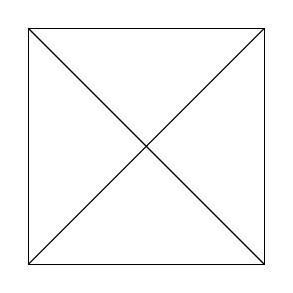
\begin{tikzpicture}
        \draw (0,0) rectangle (3,3);
        \draw (0,0)--(3,3);
        \draw (0,3)--(3,0);
    \end{tikzpicture}
    \end{minipage}
    \begin{minipage}[t]{0.45\textwidth}
    \centering
    \caption{错误的单形剖分}
    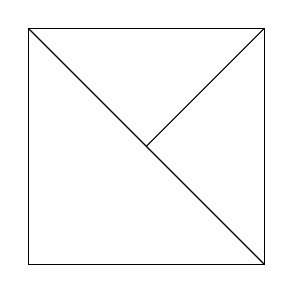
\begin{tikzpicture}
        \draw (0,0) rectangle (3,3);
        \draw (0,3)--(3,0);
        \draw (1.5,1.5)--(3,3);
    \end{tikzpicture}
    \end{minipage}
\end{figure}
有了空间划分$\mathscr{T}_{h}$后,定义在该划分空间上的分片多项式即可构成子空间$V_{h}\le V$。

\subsection{离散线性方程组与求解}
若$\dim(V_{h})=N$,设$\phi_{1},\phi_{2},\cdots,\phi_{N}$为$V_{h}$上的一组基函数,设
\begin{equation}
    u_{h}(x)=\sum_{i=1}^{N}u_{i}\phi_{i}(x),v_{h}(x)=\sum_{i=1}^{N}v_{i}\phi_{i}(x),
\end{equation}
代入\eqref{eq:GalerkinGeneral}, 我们有:
\begin{equation}
    \sum_{i=1}^{N}a(\phi_{i},\phi_{j})u_{i}=f(\phi_{j}),
\end{equation}
这是一个线性系统,求解该系统即可得到$u(x)$的近似值$u_{h}(x)$(事实上是一个分片多项式)。类似对ode边值问题的讨论,我们依旧可以称矩阵$K=(a(\phi_{i},\phi_{j}))_{ij}$为\textbf{刚度矩阵},$F=(f_{j})_{j=1}^{N}$为\textbf{负载向量}。

如果$a(\cdot,\cdot)$是对称的,Galerkin方法和Ritz方法等价。

对于刚度矩阵$K$,我们有下面的结论:
\begin{proposition}
    设$a(\cdot,\cdot):V\times V\rightarrow \mathbb{R}^{n}$是对称且V-椭圆的双线性形式,那么对应Galerkin-Ritz变分问题近似解的刚度矩阵$K$是对称正定的。
\end{proposition}
\begin{proof}
    对称性由$a(\cdot,\cdot)$的对称性可即刻得到。对于正定性,取$v\in\mathbb{R}^{n}$,记
    \begin{equation}
        v_{h}(x)=\sum_{i=1}^{N}v_{i}\phi_{i}(x),
    \end{equation}
    那么:
    \begin{equation}
        v^{t}Kv=a(v_{h},v_{h})\ge a\norm{v_{h}}^{2}\ge 0.
    \end{equation}
    该式取等号当且仅当$v_{h}=0$,即$v=0$。由此,矩阵$K$是正定的。
\end{proof}
\begin{remark}
    上面的性质保证了在变分问题的左侧项$a(\cdot,\cdot)$满足一定条件的情况下,其对应的离散化线性方程组的解存在唯一,且可以通过针对正定矩阵的算法进行求解。
\end{remark}
以上推导均需要满足\textbf{Lax-Milgram引理},因此需要$V_{h}$是$V$的子空间,这种有限元方法被称为\textbf{协调有限元方法}。

对于一个具体的问题,$V=H^{1}(\Omega)$,那么$V_{h}$中的分段多项式也必须在$H^{1}(\Omega)$中。这就要求我们对分段多项式在单元交界处的行为给出一些额外的条件。下面两个定理说明了分片多项式成为$V_{h}$中元素的充要条件。

\begin{theorem}
    设$v\in H^{1}(T),\forall T\in\mathscr{T}_{h}$,且$v\in C^{0}(\bar{\Omega})$,则$v\in H^{1}(\Omega)$。
\end{theorem}
\begin{proof}
    只需要证明$v$的广义导数$D_{i}v\in L^{2}(\Omega)$,即:
    \begin{equation}
        \label{eq:GeneralL2}
        -\int_{\Omega}D_{i}v\cdot\phi\dif x=\int_{\Omega}v\cdot\partial_{i}\phi\dif x,\forall\phi\in D(\Omega).
    \end{equation}
由于$v\in C^{0}(\bar\Omega)$,且$v$在每个单元$T$上均为多元多项式,在每个单元$T$上运用Gauss-Green公式,有:
\begin{equation}
    \label{eq:GaussGreen4GL2}
    \int_{\Omega}v\cdot\partial_{i}\phi\dif x=\sum_{T\in\mathscr{T}_{h}}\int_{T}v\cdot\partial_{i}\phi\dif x=-\sum_{T}\int_{T}D_{i}v\cdot\phi\dif x+\sum_{T}\int_{\partial T}v\phi\cdot n_{i}\dif s.
\end{equation}
$n_{i}$表示单位法向量在第$i$个维度下的投影。由\eqref{eq:GaussGreen4GL2},要证\eqref{eq:GeneralL2},即证
\begin{equation}
    \label{eq:BoundaryCond}
    \sum_{T}\int_{\partial T}v\phi\cdot n_{i}\dif s=0.
\end{equation}
根据我们选取单元$T$的第五点要求,取$T_{0}\in\partial T$,有两种情况:
\begin{itemize}
    \item $T_{0}$是区域$\Omega$的边界:由$\phi\in D(\Omega)$,即$\phi|_{\partial\Omega}=0$,可知$\int_{T_{0}}v\phi\cdot n_{i}\dif s=0$。
    \item $T_{0}$是两个单元$T_{a}$和$T_{b}$的交线。此时积分式\eqref{eq:BoundaryCond}中有关线段$T_{0}$的积分表达式为
    \begin{equation}
        \label{eq:EliminateEdge}
        \int_{T_{0}\in T_{a}}v\phi\cdot n_{i}\dif s+\int_{T_{0}\in T_{b}}v\phi\cdot n_{i}\dif s.
    \end{equation}
\end{itemize}
    由于在$T_{a}$和$T_{b}$上,线段$T_{0}$位置相同,法向量方向相反,从而\eqref{eq:EliminateEdge}的值为0。故\eqref{eq:BoundaryCond}得证,即\eqref{eq:GeneralL2}成立。
\end{proof}
\begin{theorem}
    设$v|_{T}\in C^{0}(T),\forall T\in\mathscr{T}_{h}$,且$v\in H^{1}(\Omega)$,则$v\in C^{0}(\bar{\Omega})$。
\end{theorem}
\begin{proof}
    如果$v$在两个相邻单元$e$和$e'$上不连续,即在其公共边$\gamma$上$v|_{e}-v|_{e'}$不恒为0。无妨其在$\gamma$上的某段处为正,作开集$U$使得$U\subset e\cap e'$,且$v|_{e}-v|_{e'}>0$在$U\cap\gamma$上成立,则作函数$\phi\in D(U)$使得在supp$(\phi)$上$\phi>0$。如果$v\in H^{1}(\Omega)$,根据$H^{1}(\Omega)$广义函数的定义,必定有:
    \begin{equation}
        \int_{U\cap\gamma}(v|_{e}-v|_{e'})\cdot\phi\cdot n_{i}^{e}\dif s=0.
    \end{equation}
    这与前面的假定相矛盾。
\end{proof}
\begin{remark}
    上面两个定理要求:我们求得的有限元逼近解必须在整个区域内是连续的。
\end{remark}
\section{二维情形}
在本节中,我们着眼于$\Omega\subset\mathbb{R}^{2}$,讨论区域$\Omega$的三角划分,以及定义在该划分上的分片多项式函数。

首先,我们讨论\textbf{定义在三角形有界区域上的}多项式函数。
\subsection{重心坐标}
一个很容易想到的思路是,依据三角形上某些点(例如三个顶点)处的函数取值,插值得到一个多元多项式。但如果采用直角坐标,插值多项式的表达式不免会显得非常麻烦。如果能通过一些合理的坐标变换,将一般三角形区域转化为等腰直角三角形区域,则可以大大降低该区域上插值多项式形式的复杂性。这就是引入\textbf{重心坐标}的原因。
\begin{figure}[H]
    \caption{重心坐标变换}
        \centering
        \begin{tikzpicture}
            \draw (0,0)--(1,3);
            \draw (1,3)--(2,2);
            \draw (2,2)--(0,0);
            \draw [->] (3,1.5)--(8,1.5);
            \draw (9,0)--(12,0);
            \draw (12,0)--(9,3);
            \draw (9,3)--(9,0);
        \end{tikzpicture}
\end{figure}
\begin{definition}{重心坐标}
    考虑平面上的三角形$\triangle A_{1}A_{2}A_{3}$,顶点编号为逆时针,设点$P(x,y)$落在三角形内部,则定义点$P$的\textbf{重心坐标}$(\lambda_{1},\lambda_{2},\lambda_{3})$为:
    \begin{equation}
        \lambda_{1}=\frac{m(\triangle PA_{2}A_{3})}{m(\triangle A_{1}A_{2}A_{3})},\lambda_{2}=\frac{m(\triangle PA_{1}A_{3})}{m(\triangle A_{1}A_{2}A_{3})},\lambda_{3}=\frac{m(\triangle PA_{1}A_{2})}{m(\triangle A_{1}A_{2}A_{3})}.
    \end{equation}
    其中$m$表示区域的测度,在这里表示的是三角形的面积。
\end{definition}
根据定义,下面的表达式是显然的:
\begin{equation}
    \label{eq:burycenterCoordProp}
    \lambda_{i}(A_{j})=\delta_{ij}.
\end{equation}
所以,定义在$\triangle A_{1}A_{2}A_{3}$的线性函数$u$可以表示为:
\begin{equation}
    u(x,y)=u(A_{1})\lambda_{1}(x,y)+u(A_{2})\lambda_{2}(x,y)+u(A_{3})\lambda_{3}(x,y).
\end{equation}
分别取$u(x,y)=x$,$u(x,y)=y$,$u(x,y)=1$,代入上式,可得下面的性质:
\begin{proposition}{直角坐标与重心坐标的关系}
   记$A_{i}$的坐标为$(x_{i},y_{i})$,$\triangle A_{1}A_{2}A_{3}$上直角坐标和重心坐标的关系式如下:
   \begin{equation}
    \left\{
        \begin{aligned}
            x&=x_{1}\lambda_{1}+x_{2}\lambda_{2}+x_{3}\lambda_{3}\\
            y&=y_{1}\lambda_{1}+y_{2}\lambda_{2}+y_{3}\lambda_{3}\\
            1&=\lambda_{1}+\lambda_{2}+\lambda_{3}.\\
        \end{aligned}
    \right.
   \end{equation} 
\end{proposition}
重心坐标有许多非常棒的性质,可以大大简化三角形区域上的函数计算。
\begin{proposition}{重心坐标的性质}
    \begin{enumerate}
        \item 三角形三顶点$A_{1},A_{2},A_{3}$,重心$G$的坐标分别为:
        \begin{equation}
            A_{1}(1,0,0), A_{2}(0,1,0), A_{3}(0,0,1), G(\frac{1}{3},\frac{1}{3},\frac{1}{3}).
        \end{equation}
        \item 三角形三边的方程:
        \begin{equation}
            A_{1}A_{2}:\lambda_{3}=0; A_{2}A_{3}:\lambda_{1}=0; A_{3}A_{1}:\lambda_{2}=0.
        \end{equation}
        \item 平行于三角形某一边(如$A_{1}A_{2}$)的方程:$\lambda_{3}=c$。
        \item 任一$x,y$的$k$次多项式是$\lambda_{1},\lambda_{2},\lambda_{3}$的$k$次齐次多项式,反之亦然。
        \item 由$\lambda_{1}+\lambda_{2}+\lambda_{3}=1$知这三个变量线性相关。如果取独立变量$\lambda_{1},\lambda_{2}$,则:
        \begin{equation}
            \left\{
                \begin{aligned}
                    \pdfFrac{}{\lambda_{1}}&=(x_{1}-x_3)\pdfFrac{}{x}+(y_1-y_3)\pdfFrac{}{y},\\
                    \pdfFrac{}{\lambda_{2}}&=(x_{2}-x_3)\pdfFrac{}{x}+(y_2-y_3)\pdfFrac{}{y}.\\
                \end{aligned}
            \right.
        \end{equation}
        \item 重心坐标和直角坐标变换的Jacobi行列式为:
        \begin{equation}
            \det\left(\pdfFrac{(x,y)}{(\lambda_{1},\lambda_{2})}\right)=2m(\triangle_{e}).
        \end{equation}
        $m(\triangle_{e})$为三角形单元的面积。
        \end{enumerate}
\end{proposition}
\begin{exercise}
    证明重心坐标的上述性质。
\end{exercise}
重心坐标对简化单元上的积分计算具有重要的价值,由于重心坐标把一般的三角形映射到直角边长为1的等腰直角三角形,我们可以把一般积分区域上的求积分问题转化为三角形区域上求积分的问题。记$e$为三角单元,$\hat{e}$为变换后的等腰直角三角形,具体推导如下:
\begin{equation}
    \label{eq:changevariables}
    \begin{aligned}
        \int\int_{e}F(x,y)\dif x\dif y&=\int\int_{\hat{e}}F(\lambda_{1},\lambda_{2})\det\pdfFrac{(x,y)}{(\lambda_{1}\lambda_{2})}\dif\lambda_{1}\dif\lambda_{2}\\
        &=2m(\triangle_{e})\int_{0}^{1}\dif\lambda_{1}\int_{0}^{1-\lambda_{1}}F(\lambda_{1},\lambda_{2},1-\lambda_{1}-\lambda_2)\dif\lambda_{2}.
    \end{aligned}
\end{equation}
下面的积分等式在有限元计算中是重要的:
\begin{proposition}
    \begin{equation}
        \label{eq:monomial}
        \int\int_{e}\lambda_{1}^{m}\lambda_{2}^{n}\lambda_{3}^{k}\dif x\dif y=2m(\triangle_{e})\frac{m!n!k!}{(m+n+k+2)!}.
    \end{equation}
\end{proposition}
\begin{exercise}
    证明\eqref{eq:monomial}。
\end{exercise}
以分片线性多项式元为例,在实际计算中,插值基函数选取为:在其中一个顶点取值为1,其余顶点取值均为0的分片线性函数。其形式与一维情形的hat-function比较类似,示意图如下:
\begin{figure}[H]
    \caption{二维分片线性插值基函数}
    \centering
    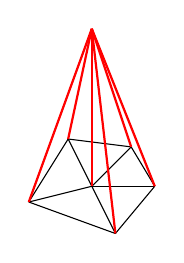
\begin{tikzpicture}
        \draw (0,0)--(0.5,0.5);
        \draw (0,0)--(0.8,0);
        \draw (0,0)--(0.3,-0.6);
        \draw (0,0)--(-0.3,0.6);
        \draw (0,0)--(-0.8,-0.2);
        \draw (0.5,0.5)--(0.8,0);
        \draw (0.8,0)--(0.3,-0.6);
        \draw (0.3,-0.6)--(-0.8,-0.2);
        \draw (-0.8,-0.2)--(-0.3,0.6);
        \draw (-0.3,0.6)--(0.5,0.5);
        \draw[color=red,thick] (0,0)--(0,2);
        \draw[color=red,thick] (0,2)--(0.5,0.5);
        \draw[color=red,thick] (0,2)--(0.8,0);
        \draw[color=red,thick] (0,2)--(0.3,-0.6);
        \draw[color=red,thick] (0,2)--(-0.3,0.6);
        \draw[color=red,thick] (0,2)--(-0.8,-0.2);
    \end{tikzpicture}
\end{figure}
\subsection{三角单元内分段多项式的形式}
本节中,我们借助重心坐标,在有合适插值条件的前提下,写出每个三角单元内部分片多项式的表达式。

如无特殊说明,本节中单元$e$指的是三角形$\triangle A_{1}A_{2}A_{3}$。
\subsubsection{线性Lagrange元}
二元线性多项式的自由度为3。要在单元$e$上确认一个线性二元多项式,需要三个插值条件,考虑在单元$e$的三个顶点处给出:
\begin{equation}
    \label{eq:LinearCond}
    u(A_{i})=u_{i},i=1,2,3.
\end{equation}
由重心坐标的性质,即
\begin{equation}
    \lambda_{i}(A_{j})=\delta_{ij},
\end{equation}
可得:
\begin{equation}
    p(x,y)=\sum_{i=1}^{3}u_{i}\lambda_{i}(x,y).
\end{equation}
这就是重心坐标下\textbf{线性Lagrange元}的表达式。
\subsubsection{完全二次Lagrange元}
$e$上的完全二次多项式可以表示为:
\begin{equation}
    p(x,y)=a_{0,0}+a_{1,0}x+a_{2,0}x^2+a_{0,1}y+a_{1,1}xy+a_{0,2}y^{2}.
\end{equation}
由表达式知共有6个自由变量,需要6个插值条件。在实际计算中,我们取三角形三个顶点以及三条边的中点作为插值节点,问题转化为求一组基函数使得$u_{i}(A_{j})=\delta_{ij}$。

插值节点如图所示:
\begin{figure}[H]
    \caption{插值节点示意,此处待完善,问题在于如何进行符号标注}
    \centering
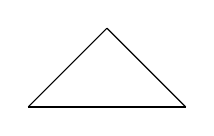
\begin{tikzpicture}
    \draw (0,0)--(2,0);
    \draw (2,0)--(1,1);
    \draw (1,1)--(0,0);
\end{tikzpicture}
\end{figure}
首先考虑构造二次多项式$p(\lambda_{1},\lambda_{2},\lambda_{3})$,使得在顶点$A_{1}$上的取值为1,在其他顶点和线段中点处取值均为0。由于$\lambda_{1}(A_{1})=1,\lambda_{1}(A_{i})=0(i\neq 1)$,可以取$\lambda_{1}$为$p$的一个因子。由于$A_{5}A_{6}$平行于$A_{2}A_{3}$,且为中点连线,故该线段的表达式为$\lambda_{1}=\frac{1}{2}$。从而$(2\lambda_{1}-1)$也是$p$的因子。此时取基函数$p(\lambda_{1},\lambda_{2},\lambda_{3})=\lambda_{1}(2\lambda_{1}-1)$,经检验可知该多项式在$A_{1}$取1,在$A_{i}(i\neq 1)$均取0。

下面考虑如何选取多项式使得中点处取值为1,其余为0。以$A_{1}A_{2}$的中点为例,在该点处,$\lambda_{1}=\lambda_{2}=\frac{1}{2},\lambda_{3}=0$。故一个比较合理的取法是$p(x,y)=4\lambda_{1}\lambda_{2}$。经验证知,该多项式满足基函数的要求。

因此,完全二次Lagrange元的表达式可以写为:
\begin{equation}
    p_{2}(x,y)=u_{1}\lambda_{1}(2\lambda_{1}-1)+u_{2}\lambda_{2}(2\lambda_{2}-1)+u_{3}\lambda_{3}(2\lambda_{3}-1)+4u_{6}\lambda_{1}\lambda_{2}+4u_{4}\lambda_{2}\lambda_{3}+4u_{5}\lambda_{3}\lambda_{1}.
\end{equation}
\subsubsection{完全三次Lagrange元}
完全三次Lagrange元需要10个插值节点,这里取三角形三个顶点,三条边上的三等分点以及三角形的重心。类似完全二次Lagrange元的讨论,完全三次Lagrange元的表达式可以写成:
\begin{equation}
    \label{eq:complete3order}
    p(x,y)=\sum_{i=1}^{3}u_{i}\frac{\lambda_{i}(3\lambda_{i}-1)(3\lambda_{i}-2)}{2}+\sum_{i\neq j}\frac{9}{2}\lambda_{i}\lambda_{j}(3\lambda_{i}-1)u_{iij}+27\lambda_{1}\lambda_{2}\lambda_{3}u_{123}.
\end{equation}
\begin{exercise}
    证明\eqref{eq:complete3order}中选取的函数确实构成一组插值基底。
\end{exercise}
\chapter{协调有限元的误差分析}
本章中,我们将借助Sobolev空间以及其上的范数,对协调有限元的求解误差进行估计。
\section{误差估计的整体流程}
经过协调有限元离散后,原微分方程边值问题对应的变分问题为:
\begin{definition}{微分方程弱形式}
    \label{def:WeakForm}
    求$u\in V$使得
    \begin{equation}
        a(u,v)=f(v),\forall v\in V.
    \end{equation}
    其中$V$是定义在$\Omega$上的函数的Hilbert空间,双线性型$a(\cdot,\cdot)$是连续且$V-$椭圆的,$f$是线性连续泛函。
\end{definition}
设$V_{h}\le V$是有限元子空间,则\textbf{有限元逼近问题}为
\begin{definition}{有限元逼近问题}
    \label{def:FEApprox}
    求$u_{h}\in V_{h}$使得
    \begin{equation}
        a(u_{h},v_{h})=f(v_{h}).
    \end{equation}
\end{definition}
直接讨论有限元逼近问题的解不太容易,讨论对应的插值问题相对容易一些。和一维有限元分析类似,高维情况下也有对应的\textbf{Cea引理}。
\begin{lemma}{Cea引理}
    \label{lem:Cea}
    设双线性型$a(\cdot,\cdot)$是连续且$V-$椭圆的,则存在$C>0$使得:
    \begin{equation}
        \norm{u-u_{h}}_{V}\le C\inf_{v_{h}\in V_{h}}\norm{u-v_{h}}_{V},
    \end{equation}
    其中$u,u_{h}$分别为准确解和有限元解。
\end{lemma}
\begin{proof}
    由于$a(\cdot,\cdot)$连续且$V-$椭圆,可知双线性型$a$可以在空间$V$上诱导一个内积。由问题\ref{def:WeakForm}和\ref{def:FEApprox}的描述可知:
    $\forall v_{h}\in V_{h},u\in V$,有$a(u-u_{h},v_{h})=0$成立。即向量$u-u_{h}$与子空间$V_{h}$关于内积$a(\cdot,\cdot)$正交。由此,我们有:
    \begin{equation}
        \norm{u-u_{h}}_{V}^{2}\le\frac{1}{\alpha}|a(u-u_{h},u-u_{h})|=\frac{1}{\alpha}|a(u-u_{h},u-v_{h})|\le\frac{M}{\alpha}\norm{u-u_{h}}_{V}\norm{u-v_{h}}_{V}.
    \end{equation}
    上式中,第一个不等号由V-椭圆性导出,第二个等号源于$u-u_{h}$与子空间$V_{h}$的正交性,第三个不等号源于双线性型的有界性。

    由此可得:
    \begin{equation}
        \norm{u-u_{h}}_{V}\le\frac{M}{\alpha}\norm{u-v_{h}}_{V}.
    \end{equation}
\end{proof}
\begin{exercise}
    试证明在\textbf{Cea引理}中常数$C$可以优化为$\sqrt{\frac{M}{\alpha}}$。
\end{exercise}
\begin{remark}
    \textbf{Cea引理}的重要意义在于将有限元的误差估计问题归结于插值误差估计问题。事实上,假定$\mathscr{T}_{h}$为空间$\Omega$的有限元划分,$\pi_{h}u$代表对函数$u$的样条插值,$\pi_{T}u$代表对函数$u$在单元$T$上的插值,那么我们有:
    \begin{equation}
        \label{eq:errorapprox}
        \inf_{v_{h}\in V_{h}}\norm{u-v_{h}}_{V}\le\norm{u-\pi_{h}u}_{V}=\left(\sum_{T\in\mathscr{T}_{h}}\norm{u-\pi_{T}u}_{V}^{2}\right)^{\frac{1}{2}}.
    \end{equation}
    由此,问题归结于估计(三角)单元$T$上的插值误差$\norm{u-\pi_{T}u}_{1,T}$。
\end{remark}
单元$T$的任意性可能会使得插值误差不好计算,所以我们需要考虑一个仿射变换$F_{T}:\hat{T}\rightarrow T$,把标准参考单元$\hat{T}:\{(x,y):x\ge 0,y\ge 0,x+y\le 1\}$变换为我们需要讨论的三角单元$T$,而后把$T$上的误差估计转化到$\hat{T}$上完成。

根据$F_{T}$,我们可以定义下面两个映射:
\begin{equation}
    \hat{v}(\hat{x}):=v(F(\hat{x}))=v(F_{T}(\hat{x}))=v(x).
\end{equation}
\begin{equation}
    \hat{\pi}_{\hat{T}}\hat{u}(\hat{x}):=\pi_{T}u(F(\hat{x}))=\pi_{T}u(x).
\end{equation}
据此我们可以写出误差估计的全流程:
\begin{enumerate}
    \item 把有限元解的误差根据Cea引理转化为插值误差。
    \item 把整体的插值误差估计转化为每个三角单元$T$上的插值误差估计。
    \item 将三角单元$T$上的插值误差转化为标准单元$\hat{T}$上的插值误差。
    \item 利用等价范数定理建立$\hat{T}$上的插值误差估计。
    \item 将标准单元$\hat{T}$上的范数$|\hat{u}|_{k+1,\hat{T}}$转化到一般单元上的范数$|u|_{k+1,T}$。
\end{enumerate}
\section{Sobolev空间上的插值误差估计}
\subsection{仿射等价元之间的范数关系}
\begin{definition}{仿射等价}
    称$\mathbb{R}^{n}$中的两个开子集$\Omega,\hat{\Omega}$是\textbf{仿射等价}的,如果存在可逆的仿射变换
    \begin{equation}
        F:F(\hat{x})=B\hat{x}+b=x\in\Omega,\forall\hat{x}\in\hat{\Omega}.
    \end{equation}
    使得$\Omega=F(\hat{\Omega})$。
\end{definition}
\begin{theorem}
    \label{thm:MAIN}
    设$\Omega$和$\hat{\Omega}$仿射等价,若$v\in W^{m,p}(\Omega)$,令
    \begin{equation}
        \hat{v}(\hat{x}):=v(F(\hat{x}))=v(x),
    \end{equation}
    则$\hat{v}\in W^{m,p}(\Omega)$且:
    \begin{equation}
        \label{eq:semiNormApprox1}
        |\hat{v}|_{m,p,\hat{\Omega}}\le C\norm{B}^{m}|\det B|^{-\frac{1}{p}}|v|_{m,p,\Omega}.
    \end{equation}
    其中$C$为仅与$m,n$有关的正常数,$\norm{B}$为矩阵$B$的Euclid范数。类似地,下面这个等式也成立:
    \begin{equation}
        \label{eq:semiNormApprox2}
        |v|_{m,p,\Omega}\le C\norm{B^{-1}}^{m}|\det B|^{\frac{1}{p}}|\hat{v}|_{m,p,\Omega}.
    \end{equation}
\end{theorem}
\begin{proof}
    先考虑$v\in C^{m}$。设$1\le p<\infty$,对$v\in C^{m}(\bar{\Omega})$,根据$\hat{v}$的定义则有$\hat{v}\in C^{m}(\bar{\hat{\Omega}})$,且对任何满足$|\alpha|=m$的多重指标$\alpha=(\alpha_{1},\cdots,\alpha_{n})$,有:
    \begin{equation}
        D^{\alpha}\hat{v}(\hat{x})=\nabla^{m}\hat{v}(\hat{x})(\xi_{1},\cdots,\xi_{m}).
    \end{equation}
    这里$\nabla^{m}\hat{v}$是$m$阶张量,$\xi_{i}$表示$\mathbb{R}^{m}$内的基向量。因此我们有:
    \begin{equation}
        \label{eq:seminorm}
        |\hat{v}|_{m,p,\hat{\Omega}}\le C_{1}(m,n)\left(\int_{\hat{\Omega}}\norm{\nabla^{m}\hat{v}(\hat{x})}^{p}\dif\hat{x}\right)^{\frac{1}{p}}
    \end{equation}
    下面讨论如何将\eqref{eq:seminorm}中的变量$\hat{x}$转化为$\Omega$内的变量$x$。利用复合函数的微分法则:
    \begin{equation}
        \nabla^{m}\hat{v}(\hat{x})(\xi_{1},\cdots,\xi_{m})=\nabla^{m}v(x)(B\xi_{1},\cdots,B\xi_{m}).
    \end{equation}
    我们有:
    \begin{equation}
        \norm{\nabla^{m}\hat{v}(\hat{x})}\le\norm{\nabla^{m}v(x)}\cdot\norm{B}^{m}=\norm{\nabla^{m}v(F(\hat{x}))}\cdot\norm{B}^{m}.
    \end{equation}
    将上式代入\eqref{eq:seminorm}右侧的表达式, 可知:
    \begin{equation}
        \int_{\hat{\Omega}}\norm{\nabla^{m}\hat{v}(\hat{x})}^{p}\dif\hat{x}\le\int_{\hat{\Omega}}\norm{\nabla^{m}v(F(\hat{x}))}\cdot \norm{B}^{mp}\dif\hat{x}=|\det(B^{-1})|\norm{B}^{mp}\int_{\Omega}\norm{\nabla^{m}v(x)}\dif x.
    \end{equation}
    又由于有界性,可得存在常数$C_{2}(m,n)$使得:
    \begin{equation}
        \norm{D^{m}v(x)}\le C_{2}(m,n)\max_{|\alpha|=m}|D^{\alpha}v(x)|.
    \end{equation}
    综合上述,可得:
    \begin{equation}
        |\hat{v}|_{m,p,\hat{\Omega}}\le C(m,n)\norm{B}^{m}|\det B|^{-\frac{1}{p}}|v|_{m,p,\Omega}.
    \end{equation}
    在$p<+\infty$的情况下,利用$C^{m}(\bar{\Omega})$在$H^{m,p}(\Omega)$中的稠密性可知,上述不等式对$v\in H^{m,p}(\Omega)$也成立。

    如果$p=+\infty$,对于$\forall v\in H^{m,\infty}(\Omega)$,有$v\in H^{m,p}(\Omega)\forall p<\infty$。根据前面的结论,$|D^{\alpha}\hat{v}|_{0,p,\hat{\Omega}}$的上界与$p$无关,因此函数$D^{\alpha}\hat{v}\in L^{\infty}(\hat{\Omega})$。由$\alpha$任意性可得$\hat{v}\in H^{m,\infty}(\hat{\Omega})$。再利用嵌入定理即证。
\end{proof}
\begin{exercise}
    用类似的方法证明等式\eqref{eq:semiNormApprox2}。
\end{exercise}
\begin{remark}
    上面的定理说明了如果$\Omega$和$\hat{\Omega}$仿射等价,则半范数$|\cdot|_{m,p,\hat{\Omega}}$和半范数$|\cdot|_{m,p,\Omega}$为等价半范数。
\end{remark}
定理5.1给出了两个范数之间的等价关系。具体的倍率则需要由$\norm{B}$和$|\det(B)|$来进行控制。而由于矩阵$B$刻画了$\Omega$和$\hat{\Omega}$几何特征的差异。为了估计$\norm{B}$和$\det(B)$,引入下列记号来描述这两个区域的几何信息:
\begin{itemize}
    \item $h$:$\Omega$的直径。
    \item $\hat{h}$:$\hat{\Omega}$的直径。
    \item $\rho$:$\Omega$最大内接球的直径。
    \item $\hat{\rho}$:$\hat{\Omega}$最大内接球的直径。
\end{itemize}
对于$\norm{B}$和$\det(B)$的控制,有下面这些结论成立:
\begin{lemma}
    \begin{equation}
        \norm{B}\le\frac{h}{\hat{\rho}},\norm{B^{-1}}\le\frac{\hat{h}}{\rho}.
    \end{equation}
\end{lemma}
\begin{lemma}
    \begin{equation}
    \det(B)=\frac{|\Omega|}{|\hat{\Omega}|}.
    \end{equation}
\end{lemma}
\begin{lemma}
    设$\sigma_{n}$是$\mathbb{R}^{n}$中单位球的体积,$\hat{\sigma}_{n}=C\frac{\sigma_{n}}{m(\hat{\Omega})}$,则:
    \begin{equation}
        C_{1}\hat{\sigma}_{n}\rho^{n}\le|\det(B)|\le C_{2}\hat{\sigma}_{n}h^{n}.
    \end{equation}
\end{lemma}
\subsection{单元上的插值误差估计}
下面的定理给出的是全空间$\Omega$上的插值误差估计。
\begin{theorem}
    设$W^{k+1,p}(\hat{\Omega})$和$W^{m,q}(\hat{\Omega})$是两个Sobolev空间,$0\le m\le k+1$,满足
    \begin{equation}
        W^{k+1,p}(\hat{\Omega})\hookrightarrow W^{m,q}(\hat{\Omega}).
    \end{equation}
    又设$\hat{\pi}_{h}$是定义在$W^{k+1,p}(\hat{\Omega})$上的有界线性算子,且保持$k$次多项式不变。又设$\Omega$和$\hat{\Omega}$仿射等价,且
    \begin{equation}
        \widehat{\pi_{h}v}=\hat{\pi}_{h}\hat{v}.
    \end{equation}
    则存在正常数$C$使得下面的不等式成立:
    \begin{equation}
        |v-\pi_{h}v|_{m,q,\Omega}\le C\left[m(\Omega)\right]^{\frac{1}{q}-\frac{1}{p}}\frac{h^{k+1}}{\rho^{m}}|v|_{k+1,p,\Omega},v\in W^{k+1,p}(\Omega).
    \end{equation}
\end{theorem}
\begin{proof}
    根据定理5.1:
    \begin{equation}
        |v-\pi_{h}v|_{m,q,\Omega}\le C(m,n)\norm{B^{-1}}^{m}|\det(B)|^{\frac{1}{q}}|\hat{v}-\widehat{\pi_{h}v}|_{m,q,\hat{\Omega}}.
    \end{equation}
    由上式,我们只需要估计$|\hat{v}-\widehat{(\pi_{h}v)}|$。由题设条件,我们知道对任意的$\hat{p}_{k}\in P_{k}(\widehat{\Omega})$,有:
    \begin{equation}
        \hat{v}-\widehat{(\pi_{h}v)}=\hat{v}-\hat{\pi}_{h}\hat{v}=(I-\hat{\pi}_{h})(\hat{v}+\hat{p}_{k}).
    \end{equation}
    从而根据等价范数定理,
    \begin{equation}
        |\hat{v}-\widehat{(\pi_{h}v)}|_{m,q,\hat{\Omega}}\le C|\hat{v}|_{k+1,p,\hat{\Omega}}.
    \end{equation}
    再利用前述引理5.2和引理5.4,可得待证等式成立。
\end{proof}
\begin{remark}
    该定理利用$v$在$W^{k+1,p}(\Omega)$上的范数,估计了插值在$W^{m,q}(\Omega)$上的误差。
\end{remark}
下面我们给出一般单元$e\in\mathcal{T}_{h}$上的插值误差估计。
\begin{theorem}
    如果下面几个条件成立:
    \begin{itemize}
        \item $\hat{v}\in H^{k+1,p}(\hat{e})$
        \item $\hat{\pi}_{\hat{e}}:H^{k+1,p}(\hat{e})\rightarrow H^{m,q}(\hat{e})$, 满足
        \begin{equation}
            \hat{\pi}_{\hat{e}}\hat{p}_{k}=\hat{p}_{k},\forall\hat{p}_{k}\in\hat{P}_{k}(\hat{e}).
        \end{equation}
        \item 对整数$k\ge 0,m\ge 0$,有下列嵌入关系:
        \begin{equation}
            \begin{aligned}
                H^{k+1,p}(\hat{e})&\hookrightarrow \bar{C}^{s}(\hat{e}),s=0,1,2\\
                H^{k+1,p}(\hat{e})&\hookrightarrow H^{m,q}(\hat{e}).\\
            \end{aligned}
        \end{equation}
        \item 对任意单元$e$,存在可逆变换$F_{e}$
        \begin{equation}
            x=F_{e}(\hat{x})=B_{e}\hat{x}+b.
        \end{equation}
        使$e=F(\hat{e})$.
    \end{itemize}
    则:
    \begin{equation}
        |v-\pi_{e}v|_{m,q,e}\le C\left[m(e)\right]^{\frac{1}{q}-\frac{1}{p}}\frac{h_{e}^{k+1}}{\rho_{e}^{m}}|v|_{k+1,p,e},v\in W^{k+1,p}(e).
    \end{equation}
\end{theorem}
\begin{proof}
    和定理5.2同理。
\end{proof}
如果剖分$\mathcal{T}_{h}$是\textbf{拟正则}的,即存在常数$\sigma>0$使得
\begin{equation}
    \frac{h_{e}}{\rho_{e}}\le\sigma,\forall e\in\mathcal{T}_{h},h_{e}>0,h_{e}\rightarrow 0.
\end{equation}
那么根据定理5.3,存在正常数$C$使得下面的插值误差估计成立:
\begin{equation}
    \label{eq:errorofeachcell}
    |v-\Pi_{e}v|_{m,q,e}\le Ch_{e}^{k+1-m+n(\frac{1}{q}-\frac{1}{p})}|v|_{k+1,p,e}.
\end{equation}
根据\eqref{eq:errorofeachcell}中的局部误差估计,推广到整体,可以得到以下推论:
\begin{corollary}
    假设定理5.3的条件满足,且剖分是拟正则的,$h$为所有单元的最大直径,则:
    \begin{equation}
        \label{eq:globalanalysis}
        |v-\Pi_{h}v|_{m,p,\Omega}\le Ch^{k+1-m}|v|_{k+1,p,\Omega},\forall v\in W^{k+1,p}(\Omega).
    \end{equation}
\end{corollary}
\begin{remark}
    可以把上面的推论5.1和一维样条插值的误差估计结果进行一些比对。
\end{remark}
\section{多边形区域上二阶问题的分析}
下面我们具体讨论二阶问题的误差估计,即区域$\Omega\in\mathbb{R}^{2}$上的变分问题。设这个二阶问题的解空间$V$满足:$H_{0}^{1}(\Omega)\subset V\subset H^{1}(\Omega)$。以下是下面的误差分析成立需要满足的一系列前提条件:
\begin{itemize}
    \item 区域划分$\mathcal{T}_{h}$是拟正则的。
    \item 有限元族$\{e,P_{e},\Sigma_{e}\}_{e\in\mathcal{T}_{h},h>0}$与一个参考元$(\hat{e},\hat{P}_{\hat{e}},\hat{\Sigma}_{\hat{e}})$仿射等价。
    \item $\{(e,P_{e},\Sigma_{e})\}$属于$C^{0}$类,即为协调元。 
\end{itemize}
\begin{remark}
    第一个条件保证了区域划分不会出现一些"过于尖锐的"三角形。第二个条件则是我们利用参考元族研究有限元族的依据。第三个条件则是利用插值估计有限元误差的基本依据。
\end{remark}
\subsection{解的$H^{1}$模误差估计}
对于$H^{1}$模的误差估计,我们可以使用Cea引理,把有限元解的误差分析转化为插值的误差分析。在前提条件满足的情况下,有下面的定理成立:
\begin{theorem}
    如果$P_{k}(\hat{e})\subset\hat{P}_{\hat{e}}\subset H^{l}(\hat{e}), H^{k+1}(\hat{e})\hookrightarrow C^{s}(\hat{e}),$,其中$0\le l\le k$,$s$是$\hat{\Sigma}_{\hat{e}}$中出现的最高阶导数,则对任意$v\in H^{k+1}(\Omega)\cap V$,有:
    \begin{equation}
        \label{eq:H1approx}
        \begin{aligned}
            &\norm{v-\Pi_{h}v}_{m,\Omega}\le Ch^{k+1-m}|v|_{k+1,\Omega},0\le m\le \min\{1,l\},\\
            &\left(\sum_{e\in\mathcal{T}_{h}}\norm{v-\Pi_{e}v}_{m,e}^{2}\right)^{\frac{1}{2}}\le Ch^{k+1-m}|v|_{k+1,\Omega},0\le m\le l.
        \end{aligned}
    \end{equation}
    其中$\Pi_{h}v$表示$v$在$V_{h}$中的分片插值。
\end{theorem}
\begin{proof}
    在表达式\eqref{eq:errorofeachcell}中,取$p=q=2$可得:
    \begin{equation}
        \norm{v-\Pi_{e}v}_{m,e}\le Ch_{e}^{k+1-m}|v|_{k+1,e}.
    \end{equation}
    由于$h$是单元直径的最大值,我们有$h_{e}\le h$,由上式求和可得:
    \begin{equation}
        \left(\sum_{e\in\mathcal{T}_{h}}\norm{v-\Pi_{e}v}_{m,e}^{2}\right)^{\frac{1}{2}}\le Ch^{k+1-m}\left(\sum_{e\in\mathcal{T}_{h}}|v|_{k+1,e}^{2}\right)^{\frac{1}{2}}=Ch^{k+1-m}|v|_{k+1,\Omega}.
    \end{equation}
    而当$0\le m\le\min\{1,l\}$时,\eqref{eq:H1approx}的第二式左边可以写成$\norm{v-\Pi_{h}v}_{m,\Omega}$,从而第一式也可得证。
\end{proof}
在定理5.4中取$l=1$,再借助Cea引理,可以得到$H^{1}$范数的估计式:
\begin{theorem}
    如果$v\in H^{k+1}(\Omega)\cap V$且定理5.4的条件成立,那么我们有下面的估计式成立:
    \begin{equation}
        \label{eq:approx}
        \norm{u-u_{h}}_{1,\Omega}\le Ch^{k}|u|_{k+1,\Omega}.
    \end{equation}
\end{theorem}
\begin{remark}
    定理5.5说明了子空间$V$选取$p$次元确实意味着有限元解的$H^{1}$误差能达到$p$阶精度。但$p$也并非越大越好。一方面高次元的计算复杂度也会大幅度上升,另一方面,定理5.5的估计式需要真实解$u$也满足$u\in H^{k+1}(\Omega)$。
\end{remark}
\section{$L^{2}$模与负模的估计}
\subsection{$L^{2}$模估计}
上面我们利用插值误差和Cea引理,估计了在$H^{1}(\Omega)$空间范数意义下的相对误差阶数。有时候我们需要对有限元解在其他范数意义下的误差进行估计,比较常用的范数是$L^{2}(\Omega)$。这时\textbf{我们不能直接用插值误差导出$L^{2}$误差,因为没有对应的Cea引理},这时我们必须要建立$u-u_{h}$的$L^{2}$误差与$H^{1}$误差的关系。下面是对应的结论,这是一维情形下Aubin-Nitsche技巧的推广。
\begin{theorem}{Aubin-Nitsche}
    设$a(\cdot,\cdot)$是连续且V-椭圆的双线性型,变分问题:求$u\in V$使得$a(u,v)=\innerprod{f}{v}\forall v$在空间$V_{h}\le V$上的有限元解为$u_{h}$,那么存在一个正常数$C$使得下列不等式成立:
    \begin{equation}
        \norm{u-u_{h}}_{0,\Omega}\le C\norm{u-u_{h}}_{1,\Omega}\sup_{g\in L^{2}(\Omega)}\left\{\frac{1}{\norm{g}_{0,\Omega}}\inf_{v_{h}\in V_{h}}\norm{\Phi-v_{h}}_{1,\Omega}\right\}.
    \end{equation}
    其中$\Phi$为共轭问题
    \begin{equation}
        a(\Phi,v)=\innerprod{g}{v}\forall v\in V_{h}
    \end{equation}
    的解。
\end{theorem}
\begin{proof}
    由$L^{2}(\Omega)$范数的定义,我们有
    \begin{equation}
        \label{eq:DefOfNorm}
        \norm{u-u_{h}}_{0,\Omega}=\sup_{g\in L^{2}(\Omega)}\frac{|\innerprod{u-u_{h}}{g}|}{\norm{g}_{0,\Omega}}.
    \end{equation}
    下面我们需要估计$|\innerprod{u-u_{h}}{g}|$。根据Lax-Milgram引理,设$V=L^{2}(\Omega)$,存在唯一的$\Phi\in V$使得:
    \begin{equation}
        \label{eq:LM}
        a(\Phi,u-u_{h})=\innerprod{g}{u-u_{h}}.
    \end{equation}
    由投影定理,$\forall v_{h}\in V_{h}$,$a(v_{h},u-u_{h})=0$。从而:
    \begin{equation}
        \innerprod{g}{u-u_{h}}=a(\Phi-v_{h},u-u_{h}).
    \end{equation}
    综合上述等式,可得:
    \begin{equation}
        \label{eq:InnerProdApprox}
        |\innerprod{u-u_{h}}{g}|=|a(u-u_{h},\Phi-v_{h})|\le C\norm{u-u_{h}}_{1}\norm{\Phi-v_{h}}_{1}\le C\norm{u-u_{h}}_{1}\inf_{v_{h}\in V_{h}}\norm{\Phi-v_{h}}_{1}.
    \end{equation}
    根据\eqref{eq:DefOfNorm}和\eqref{eq:InnerProdApprox},Aubin-Nitsche不等式成立。
\end{proof}
如果我们讨论的偏微分方程为一个二阶椭圆问题,那么其变分形式的解满足下面的正则性估计:
\begin{theorem}
    设椭圆方程
    \begin{equation}
        \mathcal{L}u:=-\sum_{i,j=1}^{2}\partial_{i}(a_{ij}(\mathbf{x})\partial_{j}u)+a_{0}(\mathbf{x})u=f(\mathbf{x}),\mathbf{x}\in\Omega.
    \end{equation}
    其中$\Omega$是凸多边形区域,其系数满足一致椭圆性条件。在赋予一定的边值条件后,该问题的变分形式为:
    \begin{equation}
        a(u,v)=\innerprod{f}{v}\forall v\in V.
    \end{equation}
    其有限元变分形式为:
    \begin{equation}
        a(u_{h},v)=\innerprod{f}{v},\forall v\in V_{h}.
    \end{equation}
    那么,变分问题的解$u$和共轭问题的解$\Phi$满足:
    \begin{equation}
        \norm{u}_{2,\Omega}\le C\norm{f}_{0,\Omega},\norm{\Phi}_{2,\Omega}\le C\norm{g}_{0,\Omega}.
    \end{equation}
\end{theorem}
    根据定理5.4,5.6和5.7,我们有下面的结论成立:
\begin{theorem}
    \begin{equation}
        \norm{u-u_{h}}_{0,\Omega}\le Ch\norm{u-u_{h}}_{1,\Omega}.
    \end{equation}
\end{theorem}
\begin{proof}
    利用不等式
    \begin{equation}
        \norm{\Phi-\Phi_{h}}_{0,\Omega}\le Ch\norm{\Phi}_{2,\Omega}\le Ch\norm{g}_{0,\Omega}.
    \end{equation}
    结合Aubin-Nitsche定理即可得证。
\end{proof}
\subsection{负模估计}
对于负模,类似于Aubin-Nitsche定理,我们有如下结论成立:
\begin{theorem}
    设$u$和$u_{h}$分别为$\Omega$上椭圆方程的广义解和有限元离散解,那么存在一个正常数$C$,使得下列不等式成立:
    \begin{equation}
        \label{eq:52}
        \norm{u-u_{h}}_{-l,\Omega}\le C\norm{u-u_{h}}_{1,\Omega}\sup_{\psi\in H_{0}^{l}(\Omega)}\left\{\frac{1}{\norm{\psi}_{l,\Omega}}\inf_{v_{h}\in V_{h}}\norm{\Psi-v_{h}}_{1,\Omega}\right\}.
    \end{equation}
    其中$\Psi$为共轭问题
    \begin{equation}
        \label{eq:conjugateprob}
        a(v,\Psi)=\innerprod{\psi}{v},\forall v\in V
    \end{equation}
    的解。
\end{theorem}
\begin{proof}
    根据定义,我们有:
    \begin{equation}
        \label{eq:54}
        \norm{u-u_{h}}_{-l,\Omega}=\sup_{\psi\in H_{0}^{l}(\Omega)}\frac{|\innerprod{u-u_{h}}{\psi}|}{\norm{\psi}_{l,\Omega}}.
    \end{equation}
    令$\Psi_{h}$为\eqref{eq:conjugateprob}的有限元解,根据方程\eqref{eq:conjugateprob}和$u-u_{h}$对空间$V_{h}$的正交性,我们可以推知:
    \begin{equation}
        \label{eq:55}
        \begin{aligned}
            \innerprod{u-u_{h}}{\psi}&=a(u-u_{h},\Psi)\\
            &=a(u-u_{h},\Psi-\Psi_{h})\\
            &\le M\norm{u-u_{h}}_{1}\norm{\Psi-\Psi_{h}}_{1}\\
            &\le C\norm{u-u_{h}}_{1}\inf_{v_{h}\in V_{h}}\norm{\Psi-v_{h}}_{1}.
        \end{aligned}
    \end{equation}
    将\eqref{eq:55}代入\eqref{eq:54},即可得\eqref{eq:52}成立。
\end{proof}
对于\eqref{eq:conjugateprob},有下面的正则性估计成立:
\begin{equation}
    \norm{\Psi}_{l+2,\Omega}\le C\norm{\psi}_{l,\Omega}.
\end{equation}
\begin{exercise}
    利用定理5.9和正则性估计证明
    下面的误差估计式:
    \begin{equation}
        \norm{u-u_{h}}_{-l,\Omega}\le Ch^{l+1}\norm{u-u_{h}}_{1,\Omega}.
    \end{equation}
\end{exercise}
\section{逆不等式}
下面我们把关注点转向有限元空间$V_{h}$本身。我们知道,对于$H_{0}^{1}(\Omega)$上的函数,我们可以用高阶模来估计低阶模,即Poincare-Friedrichs不等式:
\begin{equation}
    \norm{u}_{0,\Omega}\le C|u|_{1,\Omega},\forall u\in H_{0}^{1}(\Omega).
\end{equation}
但对于一般的函数,我们不能用低阶模来估计高阶模,例如一致有界的函数列,其导数却完全可以无界。

然而,有限元空间作为一个特殊的函数空间,我们可以在其上用低阶模来估计高阶模。这就是本节中需要讨论的\textbf{逆不等式}。

\subsection{单元上的逆不等式}
\begin{theorem}
    设$\mathcal{T}_{h}$是$\Omega$的拟正则剖分,$P(e)$是定义在单元$e\in\mathcal{T}_{h}$上的多项式空间,那么下面的逆不等式成立:
    \begin{equation}
        \begin{aligned}
            |p|_{1,e}&\le Ch_{e}^{-1}\norm{p}_{0,e},\forall p\in P(e),e\in\mathcal{T}_{h},\\
            \norm{p}_{0,\infty,e}&\le Ch_{e}^{-\frac{n}{2}}\norm{p}_{0,e},\forall p\in P(e),e\in\mathcal{T}_{h}.
        \end{aligned}
    \end{equation}
\end{theorem}
\begin{proof}
    令$\hat{e}$是标准三角单元,并存在可逆仿射变换
    \begin{equation}
        F:\hat{e}\rightarrow e, F(\hat{x})=B\hat{x}+b=x\in e,\forall\hat{x}\in\hat{e}.
    \end{equation}
    那么:根据定理\ref{thm:MAIN},有:
    \begin{equation}
        |p|_{1,e}\le C\norm{B^{-1}}|\det(B)|^{\frac{1}{2}}|\hat{p}|_{1,\hat{e}}.
    \end{equation}
    又,由于$\norm{\hat{p}}_{0,\hat{e}}$和$\norm{\hat{p}}_{1,\hat{e}}$均为$P(\hat{e})$上的范数,且在有限元空间上,因此这两个范数等价,即:
    \begin{equation}
        \norm{\hat{p}}_{1,\hat{e}}\le \hat{C}\norm{\hat{p}}_{0,\hat{e}}.
    \end{equation}
    于是:
    \begin{equation}
        \begin{aligned}
            \norm{p}_{1,e}&\le C\norm{B^{-1}}|\det(B)|^{\frac{1}{2}}\norm{\hat{p}}_{0,\hat{e}}\\
            &\le C\norm{B^{-1}}|\det(B)|^{\frac{1}{2}}|\det(B)|^{-\frac{1}{2}}\norm{p}_{0,e}\\
            &\le C\rho_{e}^{-1}\norm{p}_{0,e}\\
            &\le Ch_{e}^{-1}\norm{p}_{0,e}.
        \end{aligned}
    \end{equation}
    对于第二式,由定理\ref{thm:MAIN}可得
    \begin{equation}
        \norm{p}_{0,\infty,e}\le C\norm{\hat{p}}_{0,\infty,\hat{e}},
    \end{equation}
    而在$P(\hat{e})$上,$\norm{\hat{p}}_{0,\infty,\hat{e}}$与$\norm{\hat{p}}_{0,\hat{e}}$等价,从而:
    \begin{equation}
        \norm{\hat{p}}_{0,\infty,\hat{e}}\le\hat{C}\norm{\hat{p}}_{0,\hat{e}}.
    \end{equation}
    于是:
    \begin{equation}
        \norm{p}_{0,\infty,e}\le C\norm{\hat{p}}_{0,\hat{e}}\le C|\det(B)|^{-\frac{1}{2}}\norm{p}_{0,e}\le Ch_{e}^{-\frac{n}{2}}\norm{p}_{0,e}.
    \end{equation}
\end{proof}
\subsection{逆不等式}
\begin{definition}{拟一致条件}
    存在正常数$\nu$,使得:
    \begin{equation}
        \frac{h}{h_{e}}\le\nu,\forall e\in\mathcal{T}_{h},h\rightarrow 0.
    \end{equation}
    其中$h_{e}=\text{diam}(e)$, $h=\max_{e\in\mathcal{T}_{h}}\{h_{e}\}$.
\end{definition}
下面叙述整体区域下的逆不等式。
\begin{theorem}{逆不等式}
    设$\Omega\subset\mathbb{R}^{n}$为有界凸多边形开区域,设剖分$\mathcal{T}_{h}$满足正则性条件,仿射等价条件和拟一致条件,且:
    \begin{equation}
        \hat{P}_{\hat{e}}\subset H^{l,r}(\hat{e})\cap H^{m,q}(\hat{e}), 0\le l\le m, 1\le r,q\le \infty.
    \end{equation}
    则存在常数使得对任意$v_{h}\in V_{h}$,有:
    \begin{equation}
        \left(\sum_{e\in\mathcal{T}_{h}}|v_{h}|_{m,q,e}^{q}\right)^{\frac{1}{q}}\le\frac{C}{(h^{n})^{\max\{0,\frac{1}{r}-\frac{1}{q}\}}h^{m-l}}\left(\sum_{e\in\mathcal{T}_{h}}|v_{h}|_{l,r,e}^{r}\right)^{\frac{1}{r}}.
    \end{equation}
    其中分片多项式空间:
    \begin{equation}
        V_{h}:=\left\{v_{h}:v_{h}|_{e}\in P_{e}\leftrightarrow \hat{P}_{\hat{e}}\subset H^{l,r}(\hat{e})\cap H^{m,q}(\hat{e})\right\}.
    \end{equation}
    特别地,取$\hat{P}_{\hat{e}}\subset H^{1}(\hat{e})$,且$V_{h}\subset C(\bar{\Omega})\cap H^{1}(\Omega)$,则:
    \begin{equation}
        \begin{aligned}
        |v_{h}|_{0,\infty,\Omega}&\le Ch^{-\frac{n}{2}}|v_{h}|_{0,\Omega},\forall v_{h}\in V_{h}\\
        |v_{h}|_{1,\Omega}&\le Ch^{-1}|v_{h}|_{0,\Omega},\forall v_{h}\in V_{h}.
        \end{aligned}
    \end{equation}
\end{theorem}
证明在本笔记中按下不表。

最后,作为本节的结束,我们利用逆不等式证明两个模估计定理。
\begin{theorem}{$H^{s}$模估计}
    设$u\in H^{m}\cap H_{0}^{1}(\Omega)$为变分问题的解,$u_{h}\in V_{h}$为有限元逼近问题的解,那么有下面的最佳误差估计:
    \begin{equation}
        \norm{u-u_{h}}_{s,\Omega}\le Ch^{m-s}\norm{u}_{m,\Omega},0\le s\le m-1.
    \end{equation}
\end{theorem}
\begin{proof}
    我们只证明$1\le s\le m-1$的情形。根据定理5.11,取$m=s$,$r=q=2$,$l=1$,对任意$v_{h}\in V_{h}$,有:
    \begin{equation}
        |v_{h}|_{s,\Omega}=\left(\sum_{e\in\mathcal{T}_{h}}|v_{h}|_{s,e}^{2}\right)^{\frac{1}{2}}\le Ch^{1-s}\left(\sum_{e\in\mathcal{T}_{h}}|v_{h}|_{1,e}^{2}\right)^{\frac{1}{2}}\le Ch^{1-s}|v_{h}|_{1,\Omega},s\ge 1.
    \end{equation}
    于是:
    \begin{equation}
        \begin{aligned}
            \norm{u-u_{h}}_{s,\Omega}&\le\norm{u-\Pi_{h}u}_{s,\Omega}+\norm{u_{h}-\Pi_{h}u}_{s,\Omega}\\
            &\le\norm{u-\Pi_{h}u}_{s,\Omega}+Ch^{1-s}\norm{u_{h}-\Pi_{h}u}_{1,\Omega}\\
            &\le\norm{u-\Pi_{h}u}_{s,\Omega}+Ch^{1-s}(\norm{u-\Pi_{h}u}_{1,\Omega}+\norm{u-u_{h}}_{1,\Omega}).
        \end{aligned}
    \end{equation}
    利用插值逼近定理,可知
    \begin{equation}
        \begin{aligned}
            \norm{u-\Pi_{h}u}_{s,\Omega}&\le C_{1}h^{m-s}\norm{u}_{m,\Omega},\\
            \norm{u-\Pi_{h}u}_{1,\Omega}&\le C_{2}h^{m-1}\norm{u}_{m,\Omega}.
        \end{aligned}
    \end{equation}
    由$H^{1}$模估计可知:
    \begin{equation}
        \norm{u-u_{h}}_{1,\Omega}\le C_{3}h^{m-1}\norm{u}_{m,\Omega}.
    \end{equation}
    综上所述,
    \begin{equation}
        \norm{u-u_{h}}_{s,\Omega}\le Ch^{m-s}\norm{u}_{m,\Omega}.
    \end{equation}
\end{proof}
\begin{theorem}{最大模估计}
    设$\Omega$的剖分是拟正则的,$|\alpha|=s<m-1$,有限元解$u_{h}$具有如定理5.12所述的估计,则$u_{h}$有下面的最大模估计:
    \begin{equation}
        \max_{\Omega}|D^{\alpha}(u-u_{h})|\le Ch^{m-1-s}\norm{u}_{m,\Omega}.
    \end{equation}
\end{theorem}
\begin{proof}
    设$\Pi_{h}u$是$u$的$m-1$次插值函数,在单元$e_{0}$上达到$\max_{\Omega}|D^{\alpha}(u-u_{h})|$,则:
    \begin{equation}
        \max_{\Omega}|D^{\alpha}(u-u_{h})|\le\max_{\Omega}|D^{\alpha}(u-\Pi_{h}u)|+\max_{\Omega}|D^{\alpha}(\Pi_{h}u-u_{h})|.
    \end{equation}
    由插值误差分析公式可知:
    \begin{equation}
        \max_{\Omega}|D^{\alpha}(u-\Pi_{h}u)|=\max_{e_{0}}|D^{\alpha}(u-\Pi_{h}u)|\le Ch^{m-1-s}\norm{u}_{m,e_{0}}\le Ch^{m-1-s}\norm{u}_{m,\Omega}.
    \end{equation}
    令$v_{h}=\Pi_{h}u-u_{h}$,则由逆不等式,有:
    \begin{equation}
        |v_{h}|_{s,\Omega}=\left(\sum_{e\in\mathcal{T}_{h}}|v_{h}|_{s,e}^{2}\right)^{\frac{1}{2}}\le Ch^{-s}\left(\sum_{e\in\mathcal{T}_{h}}|v_{h}|_{0,e}^{2}\right)^{\frac{1}{2}}\le Ch^{-s}|v_{h}|_{0,\Omega}.
    \end{equation}
    再由逆不等式,有
    \begin{equation}
        \max_{\Omega}|D^{\alpha}v_{h}|\le Ch^{m-1-s}\norm{u}_{m,\Omega}.
    \end{equation}
    综上,最大模估计式得证。
\end{proof}
\chapter{抛物型方程的有限元求解与分析}
前面的章节中我们主要讨论的是椭圆方程的有限元解法以及其求解误差的分析。在本章中,我们转而关注抛物型方程的有限元求解与分析。在抛物型方程的有限差分算法(MOL)中,我们的思路是先对空间进行离散形成一个常微分方程组,再对生成的常微分方程组进行时间积分求解。有限元求解抛物型方程的过程中也可以借鉴这一思路,即先固定时间参数$t$,在空间上给出变分问题的形式,然后转化为一个常微分方程组,最后通过时间积分解决问题。

本章中,如无特殊说明,讨论的微分方程均为如下二维热传导方程:
\begin{equation}
    \label{eq:heat_eq}
    \left\{
        \begin{aligned}
            &u_{t}-\Delta u=f(\mathbf{x},t),(\mathbf{x},t)\in\Omega\times[0,+\infty),\\
            &u(\mathbf{x},t)=0,(\mathbf{x},t)\in\partial\Omega\times[0,+\infty),\\
            &u(\mathbf{x},0)=u_{0}(\mathbf{x}),\mathbf{x}\in\Omega.\\
        \end{aligned}
    \right.
\end{equation}
在方程\eqref{eq:heat_eq}中,要求$\Omega\subset\mathbb{R}^{2}$为有界区域,而$\Gamma:=\partial\Omega$为$\Omega$的光滑边界。

\section{空间离散(半离散)}
本节着重介绍有限元求解抛物型方程的半离散算法,以及半离散解的$L^{2}(\Omega)$范数估计。

\subsection{离散过程}
第四章里我们讨论了有限元求解微分方程的一般流程:
\begin{enumerate}
    \item 寻求原问题的变分形式。
    \item 对区域$\Omega$进行剖分。
    \item 构造有限元子空间$V_{h}$。
    \item 利用问题的变分形式建立有限元方程组。
    \item 对离散后的有限元方程组(本质上是一个线性方程组)进行求解。
\end{enumerate}
本节中,我们用同样的流程来分析热传导方程\eqref{eq:heat_eq}。

设$v\in H_{0}^{1}(\Omega)$为测试函数,$t$看作一个给定的常数,在\eqref{eq:heat_eq}的第(1)式两边同乘$v$,在$\Omega$上积分得:
\begin{equation}
    \label{eq:int_test}
    \int_{\Omega}(u_{t}v-v\Delta u)\dif\mathbf{x}=\int_{\Omega}f(\mathbf{x},t)v(\mathbf{x})\dif\mathbf{x}.
\end{equation}
由于$v|_{\partial\Omega}\equiv 0$,利用格林公式可得:
\begin{equation}
    \int_{\Omega}u_{t}v\dif\mathbf{x}+\int_{\Omega}\nabla u\cdot\nabla v\dif\mathbf{x}=\int_{\Omega}fv\dif\mathbf{x}.
\end{equation}
我们定义以下符号:
\begin{equation}
    B(u,v):=\int_{\Omega}\nabla u\cdot\nabla v\dif\mathbf{x},\innerprod{f}{v}:=\int_{\Omega}f(\mathbf{x},t)v(\mathbf{x})\dif\mathbf{x}.
\end{equation}
由此可得热传导方程的\textbf{变分形式}:
\begin{definition}
    \label{def:variate_heat}
    热传导方程的变分形式为:对每个固定的$t\in[0,+\infty)$,求$u(t)\in H_{0}^{1}(\Omega)$使得:
    \begin{equation}
        \left\{
            \begin{aligned}
                &\innerprod{u_{t}}{v}+B(u,v)=\innerprod{f}{v},\forall v\in H_{0}^{1}(\Omega)\\
                &u(\mathbf{x},0)=u_{0}(\mathbf{x})\\
            \end{aligned}
        \right.
    \end{equation}
\end{definition}
对$\Omega$的剖分可以参考椭圆方程求解时的剖分方式,即三角剖分$\mathcal{T}_{h}$。记$\Omega_{h}=\cup_{e\in\mathcal{T}_{h}}e$,其中$h$为三角剖分的最大直径。我们可以假定$\mathcal{T}_{h}$是拟一致的划分,此时每个单元$e$的面积有下界$Ch^{2}$。

由剖分$\Omega_{h}$,我们可以构造$H_{0}^{1}(\Omega)$的有限元子空间$V_{h}$如下:
\begin{equation}
    V_{h}:=\left\{v_{h}|v_{h}\in C(\bar\Omega),v_{h}|_{e}=p_{k}(\mathbf{x}),v_{h}(\mathbf{x})=0\text{ if }\mathbf{x}\notin\Omega_{h}\right\}.
\end{equation}
根据如上所述的区间划分和有限元子空间$V_{h}$定义,可得\eqref{eq:heat_eq}的半离散变分问题:
\begin{definition}
    \label{def:half-discretize_variate}
    对每个固定的$t\in [0,+\infty)$,求$u_{h}(t)\in V_{h}$使得:
    \begin{equation}
        \label{eq:half-discretize}
        \left\{
            \begin{aligned}
                &\innerprod{u_{h,t}}{v}+B(u_{h},v)=\innerprod{f}{v},\forall v\in H_{0}^{1}(\Omega)\\
                &u_{h}(\mathbf{x},0)=u_{0h}(\mathbf{x})\\
            \end{aligned}
        \right.        
    \end{equation}
\end{definition}
\eqref{eq:half-discretize}的解称为变分形式\ref{def:variate_heat}的\textbf{半离散解}。 

下面讨论如何给出$u_{h}(t)$满足的常微分方程。设空间$V_{h}$有一组基函数为$\{\varphi_{i}(\mathbf{x})\}$,对任意$u_{h}(t)\in V_{h}$进行Fourier展开,得:
\begin{equation}
    \label{eq:FourierExpension}
    u_{h}(t)=\sum_{i=1}^{N}\alpha_{i}(t)\varphi_{i}(\mathbf{x}).
\end{equation}
此时半离散问题\eqref{eq:half-discretize}可以转化为以下常微分方程组:
\begin{equation}
    \label{eq:discretized_ode}
    \left\{
        \begin{aligned}
            &\sum_{i=1}^{N}\innerprod{\varphi_{i}}{\varphi_{j}}\alpha_{i}'(t)+\sum_{i=1}^{N}B(\varphi_{i},\varphi_{j})\alpha_{i}(t)=\innerprod{f}{\varphi_{j}}.\\
            &\alpha_{i}(0)=\gamma_{i}.
        \end{aligned}
    \right.
\end{equation}
其中$\gamma_{i}$为初值$u_{0h}(\mathbf{x})$关于基底$\{\varphi_{i}(\mathbf{x})\}$展开的Fourier系数。如果引入下列矩阵记号:
\begin{equation}
    \begin{aligned}
        &\mathbf{A}:=(\innerprod{\varphi_{i}}{\varphi_{j}})\\
        &\mathbf{B}:=(B(\varphi_{i},\varphi_{j})),\mathbf{\alpha}(t):=(\alpha_{1}(t),\cdots,\alpha_{N}(t))^{T}\\
        &F(t):=(\innerprod{f}{\varphi_{1}},\cdots,\innerprod{f}{\varphi_{N}})^{T}, \mathbf{\gamma}:=(\gamma_{1},\cdots,\gamma_{N})^{T},
        \end{aligned}
\end{equation}
那么方程组\eqref{eq:discretized_ode}可以改写为:
\begin{equation}
    \left\{
        \begin{aligned}
            &\mathbf{A}\mathbf{\alpha}'(t)+\mathbf{B}\mathbf{\alpha}(t)=\mathbf{F},\\
            &\mathbf{\alpha}(0)=\mathbf{\gamma}.
        \end{aligned}
    \right.
\end{equation}
其中$\mathbf{A}$被称为\textbf{质量矩阵},$\mathbf{B}$被称为\textbf{刚度矩阵}。由ode理论可知,该微分方程存在唯一解。
\subsection{半离散解的误差}
本节中我们估计上述半离散解的求解误差。在分析时,我们假定求解常微分方程的过程不引入任何误差,即\eqref{eq:discretized_ode}的解是精确的。

在分析之前,我们假定有限元空间$V_{h}$有下面的逼近性质:
\begin{proposition}
    \begin{equation}
        \begin{aligned}
            &\inf_{\chi\in V_{h}}\left\{\norm{v-\chi}_{0,\Omega}+h\norm{\nabla(v-\chi)}_{0,\Omega}\right\}\le Ch^{s}\norm{v}_{s,\Omega},\\
            &1\le s\le k+1, k\ge 1, \forall v \in H^{s}(\Omega)\cap H_{0}^{1}(\Omega).
        \end{aligned}
    \end{equation}
\end{proposition}
\begin{remark}
    上面的性质体现了有限元空间$V_{h}$确实可以较好地逼近函数空间$H^{s}(\Omega)\cap H_{0}^{1}(\Omega)$。
\end{remark}
在讨论半离散问题有限元解的$L^{2}(\Omega)$-模估计前,我们先引入一个\textbf{椭圆投影算子}。
\begin{definition}{椭圆投影算子}
    椭圆投影算子$P_{h}:H_{0}^{1}(\Omega)\rightarrow V_{h}$对任意$u\in H_{0}^{1}(\Omega)$,满足:
    \begin{equation}
        B(P_{h}u,\chi)=B(u,\chi),\forall \chi\in V_{h}.
    \end{equation}
\end{definition}
\begin{remark}
    椭圆投影算子可以看作在以$B(\cdot,\cdot)$为内积的Hilbert空间下,函数空间$H_{0}^{1}(\Omega)$到空间$V_{h}$的投影。
\end{remark}
下面讨论椭圆投影算子的性质。对于一个满足逼近性质的有限元空间$V_{h}$,有下面的引理成立:
\begin{lemma}
    \label{lem:proj}
    设$v\in H^{s}(\Omega)\cap H_{0}^{1}(\Omega)$,$1\le s\le k+1$,则:
    \begin{equation}
        \norm{P_{h}v-v}_{0,\Omega}+h\norm{\nabla(P_{h}v-v)}_{0,\Omega}\le Ch^{s}\norm{v}_{s,\Omega}.
    \end{equation}
\end{lemma}
\begin{remark}
    上面引理保证了当$V_{h}$满足逼近性质时,$P_{h}v$是对$v$的一个好的逼近。
\end{remark}
\begin{proof}
    证明分两步,先估计$\norm{\nabla(P_{h}v-v)}_{0,\Omega}$,再估计$\norm{P_{h}v-v}_{0,\Omega}$。根据投影算子的性质,我们有如下不等式成立:
    \begin{equation}
        \label{eq:ineq_proj}
        \begin{aligned}
            \norm{\nabla(P_{h}v-v)}_{0,\Omega}^{2}&=\innerprod{\nabla(P_{h}v-v)}{\nabla(P_{h}v-v)}\\
            &=\innerprod{\nabla(P_{h}v-v)}{\nabla(\chi-v)}\forall\chi\in V_{h}\\
            &\le\norm{\nabla(P_{h}v-v)}_{0,\Omega}\norm{\nabla(\chi-v)}_{0,\Omega}\\
        \end{aligned}
    \end{equation}
    从而我们有$\norm{\nabla(P_{h}v-v)}_{0,\Omega}\le\norm{\nabla(\chi-v)}_{0,\Omega}$。又由逼近性质,有:
    \begin{equation}
        \label{eq:estimate_2}
        \norm{\nabla(P_{h}v-v)}_{0,\Omega}\le \inf_{\chi\in V_{h}}\norm{\nabla(v-\chi)}_{0,\Omega}\le Ch^{s-1}\norm{v}_{s,\Omega}.
    \end{equation}
    对于$\norm{P_{h}v-v}$的估计,我们没法直接使用投影的性质,因此我们需要利用一些技巧来提升$(P_{h}v-v)$的导数阶数。根据第二格林公式,我们可以试着讨论$P_{h}v-v$与一个标量场$\Delta w$的内积,来得到$\norm{P_{h}v-v}$的估计。而要使得$-\Delta w=P_{h}v-v$,这就导出了一个椭圆方程。

    因此我们需要讨论如下辅助问题。设$g\in L^{2}(\Omega)$,考虑下面的椭圆方程:
    \begin{equation}
        \label{eq:elliptic_aux}
        \left\{
            \begin{aligned}
                -\Delta w&=g,\\
                w|_{\partial\Omega}&=0.\\
            \end{aligned}
        \right.
    \end{equation}
    根据椭圆方程的适定性和Poincare-Friedriches不等式,该椭圆方程存在唯一解$w$,且满足不等式
    \begin{equation}
        \norm{w}_{2,\Omega}\le C\norm{\Delta w}_{0,\Omega}=C\norm{g}_{0,\Omega}.
    \end{equation}
    于是:
    \begin{equation}
        \begin{aligned}
            \innerprod{P_{h}v-v}{g}&=-\innerprod{P_{h}v-v}{\Delta w}\\
            &=\innerprod{\nabla(P_{h}v-v)}{\nabla w}\\
            &=\innerprod{\nabla(P_{h}v-v)}{\nabla (w-P_{h}w)}\\
            &\le\norm{P_{h}v-v}_{0,\Omega}\norm{\nabla(w-P_{h}w)}_{0,\Omega}\\
            &\le Ch^{s}\norm{v}_{s,\Omega}\norm{w}_{2,\Omega}\le Ch^{s}\norm{v}_{s,\Omega}\norm{g}_{0,\Omega}.
        \end{aligned}
    \end{equation}
    特别地,取$g=P_{h}v-v$,可得$\norm{P_{h}v-v}_{0,\Omega}\le Ch^{s}\norm{v}_{s,\Omega}$。

    综上,引理成立。
\end{proof}
下面的定理利用投影算子,讨论了有限元解$u_{h}$与真实解$u$的误差的$L^{2}$-模估计。
\begin{theorem}{$L^{2}$-模估计}
    设$u(\mathbf{x},t)$为\eqref{eq:heat_eq}的解,$u_{h}(t)$为其在$V_{h}$上的有限元近似解,且$u(\mathbf{x},t)\in H^{k+1}(\Omega)\cap H_{0}^{1}(\Omega)$,则有:
    \begin{equation}
        \norm{u_{h}(t)-u(\mathbf{x},t)}_{0,\Omega}\le \norm{u_{0h}-u_{0}}_{0,\Omega}+Ch^{k+1}\{\norm{u_{0}}_{k+1,\Omega}+\int_{0}^{t}\norm{u_{t}}_{k+1,\Omega}\dif s\}.
    \end{equation}
\end{theorem}
\begin{remark}
    抛物方程有限元半离散解的误差由两部分组成,第一部分是估计初值时产生的误差,第二部分是演化过程中的误差。由上面的定理可以看出,如果需要让抛物方程的有限元半离散解达到四阶精度,则至少需要三次多项式单元。
\end{remark}
\begin{proof}
    证明分三步完成。

    第一步:利用投影算子将误差分割为两部分。
    \begin{equation}
        u_{h}(t)-u(\mathbf{x},t)=(u_{h}(t)-P_{h}u)+(P_{h}u-u):=\theta(t)+\rho(t).
    \end{equation}
    $\rho(t)$表示将真实解投影到解空间$V_{h}$上产生的误差,而$\theta(t)$则表示在解空间上近似$P_{h}u$产生的误差。

    第二步:估计$\rho(t)$。

    利用引理\ref{lem:proj},取$s=k+1$,我们有:
    \begin{equation}
        \begin{aligned}
            \norm{\rho(t)}_{0,\Omega}&=\norm{P_{h}u-u}_{0,\Omega}\\
            &\le Ch^{k+1}\norm{u}_{k+1,\Omega}\\
            &\le Ch^{k+1}\norm{u_{0}+\int_{0}^{t}u_{t}\dif t}_{k+1,\Omega}\\
            &\le Ch^{k+1}\left\{
                \norm{u_{0}}_{k+1,\Omega}+\int_{0}^{t}\norm{u_{t}}_{k+1,\Omega}\dif t
            \right\}.
        \end{aligned}
    \end{equation}

    第三步:估计$\theta(t)$。首先我们需要推导$\theta$满足的方程。 

    $\forall \chi\in V_{h}$,我们有:
    \begin{equation}
        \begin{aligned}
            \innerprod{\theta_{t}}{\chi}+\innerprod{\nabla\theta}{\nabla\chi}&=\innerprod{u_{h,t}}{\chi}-\innerprod{P_{h}u_{t}}{\chi}+\innerprod{\nabla u_{h}}{\nabla\chi}-\innerprod{\nabla P_{h}u}{\nabla\chi}\\
            &=\innerprod{f}{\chi}-\innerprod{P_{h}u_{t}}{\chi}-\innerprod{\nabla u}{\nabla \chi}\\
            &=\innerprod{u_{t}-P_{h}u_{t}}{\chi}=\innerprod{-\rho_{t}}{\chi}.
        \end{aligned}
    \end{equation}
    根据投影算子的性质,$\theta(t)\in V_{h}$,那么我们可以取$\chi=\theta$,得:
    \begin{equation}
        \innerprod{\theta_{t}}{\theta}+\norm{\nabla\theta}_{0,\Omega}^{2}=-\innerprod{\rho_{t}}{\theta}.
    \end{equation}
    根据上式,可知:
    \begin{equation}
        \frac{1}{2}\difFrac{}{t}\norm{\theta}_{0,\Omega}^{2}\le\norm{\rho_{t}}_{0,\Omega}\norm{\theta}_{0,\Omega}.
    \end{equation}
    从而:
    \begin{equation}
        \difFrac{}{t}\norm{\theta}_{0,\Omega}\le\norm{\rho_{t}}_{0,\Omega}
    \end{equation}
    上式两边同时从$0$到$t$积分,可得:
    \begin{equation}
        \norm{\theta(t)}_{0,\Omega}\le \norm{\theta(0)}_{0,\Omega}+\int_{0}^{t}\norm{\rho_{t}}_{0,\Omega}\dif s.
    \end{equation}
    又:
    \begin{equation}
        \begin{aligned}
            \norm{\theta(0)}_{0,\Omega}&=\norm{u_{h}(0)-u(\mathbf{x},0)+u(\mathbf{x},0)-P_{h}u(\mathbf{x},0)}_{0,\Omega}\\
            &\le\norm{u_{0h}-u_{0}}_{0,\Omega}+\norm{u_{0}-P_{h}u_{0}}_{0,\Omega}\\
            &\le\norm{u_{0h}-u_{0}}_{0,\Omega}+Ch^{k+1}\norm{u_{0}}_{k+1,\Omega}.
        \end{aligned}
    \end{equation}
    并且
    \begin{equation}
        \norm{\rho_{t}}_{0,\Omega}\le Ch^{k+1}\norm{u_{t}}_{k+1,\Omega}.
    \end{equation}
    综合上述,结论得证。
\end{proof}
如果初值近似也为$k+1$阶的,那么$L^{2}$-模估计可以简化为:
\begin{equation}
    \norm{u_{h}(t)-u(\mathbf{x},t)}_{0,\Omega}\le Ch^{k+1}\left\{
        \norm{u_{0}}_{k+1,\Omega}+\int_{0}^{t}\norm{u_{t}}_{k+1,\Omega}\dif s
    \right\}.
\end{equation}
我们可以用类似的技巧证明下面的梯度估计定理:
\begin{theorem}{梯度估计}
    设$u$为\eqref{eq:heat_eq}的解,$u_{h}$为其有限元解,且$u\in H^{k+1}(\Omega)\cap H_{0}^{1}(\Omega)$,则:
    \begin{equation}
        \norm{\nabla u_{h}-\nabla u}_{0,\Omega}\le\norm{\nabla u_{0h}-\nabla u_{0}}_{0,\Omega}+Ch^{k}\left\{\norm{u_{0}}_{k+1,\Omega}+\norm{u(t)}_{k+1,\Omega}+\left(\int_{0}^{t}\norm{u_{t}}_{k,\Omega}^{2}\dif s\right)^{\frac{1}{2}}\right\}.
    \end{equation}
\end{theorem}
\begin{exercise}
    完成定理6.2的证明。
\end{exercise}
\subsection{全离散与误差估计}
上面一节中我们讨论了针对热方程进行半离散的思路,并分析了半离散解的$L^{2}$误差。然而,半离散后导出的常微分方程\eqref{eq:discretized_ode}往往无法直接求得解析解,而是需要对应的ode数值算法求解。这意味着我们同样需要针对时间参数$t$对系统进行离散化处理。在本节中,我们将讨论两种不同的时间积分格式,对应的是Euler-Galerkin全离散方法和Crank-Nicolson-Galerkin全离散方法,并分析这两种算法的误差阶数。
\subsection{Euler-Galerkin方法}
和数值求解常微分方程初值问题的隐式Euler方法类似,在Euler-Galerkin算法中,我们利用向后差商来近似一阶导数,即:
\begin{equation}
    \bar{\partial}_{t}U^{m}\approx\frac{U^{m}-U^{m-1}}{\Delta t}.
\end{equation}
将向后差商的表达式代入半离散方程\eqref{eq:half-discretize},可得Euler-Galerkin全离散格式如下:
\begin{equation}
    \left\{
        \begin{aligned}
            &\innerprod{U^{m}}{\chi}+\tau B(U^{m},\chi)=\innerprod{U^{m-1}+\tau f(t_{m})}{\chi},\forall \chi\in V_{h}\\
            &U^{0}=u_{0h}\\
        \end{aligned}
    \right.
\end{equation}
\begin{remark}
    此处的$U^{m}$指$t=t_{m}$时刻解$u$的近似,其中$U^{i}\in V_{h}$,$\tau$指时间间隔,即$t_{i+1}-t_{i}=\tau$。实际计算中,利用全离散格式,一定能求解出数值近似解,因为如果$U^{m-1}$已知,等式的右端项可以计算,只需要利用待定系数法求解左端分片多项式的系数即可给出$u(t_{m})$的估计。
\end{remark}
\begin{remark}
    一个疑问:为什么时间积分方法都采用隐式格式?
\end{remark}

\chapter{有限元与数值积分}
有限元求解中,对于抽象出来的有限元变分问题:
\begin{equation}
    B(u,v)=\innerprod{f}{v}\forall v\in V_{h},
\end{equation}
通常情况下,我们无法精确计算出$B(u,v)$和$\innerprod{f}{v}$的积分值,此时我们不得不在有限元空间上使用数值积分公式。本章中,我们将会描述有限元空间上的数值积分公式,以及数值积分对有限元解误差的影响。
\section{有限元空间上的数值积分}
\begin{remark}
    本节中考虑的区域$\Omega$为二维空间$\mathbb{R}^{2}$中的多边形区域,$\mathcal{T}_{h}$为多边形区域$\Omega$的有限元划分,$e\in\mathcal{T}_{h}$表示一个单元,一般为三角形或是矩形。
\end{remark}
回忆有限元离散化问题:
\begin{equation*}
    \text{求}u_{h}\in V_{h}\text{使得}B(u_{h},v_{h})=\innerprod{f}{v_{h}},\forall v_{h}\in V_{h}.
\end{equation*}
虽然$u_{h}$和$v_{h}$都是分片多项式,但由于实际计算中,双线性形式$B$和泛函$\innerprod{f}{v}$都可能有较为复杂的形式,我们往往无法精确求得对应的积分值。为此,我们需要研究单元$e$上的数值积分公式。

第一个困难在于,单元$e$的形式可能比较多样。为此我们可以参考第四章的做法,利用仿射变换建立起标准元$\hat{e}$与一般元$e$的线性关系。

假设存在可逆仿射变换
\begin{equation}
    F_{e}(\hat{x}):=B_{e}\hat{x}+b_{e},
\end{equation}
建立$\hat{e}$到$e$之间的双射,
则对于$\varphi\in C(e)$,根据换元积分法,有:
\begin{equation}
    \int_{e}\varphi\dif x=|\det(B_{e})|\int_{\hat{e}}\varphi(F_{e}(\hat{x}))\dif\hat{x}.
\end{equation}
根据上式,我们可以通过计算$\int_{\hat{e}}\hat{\varphi}(\hat{x})\dif\hat{x}$的近似值来计算$\int_{e}\varphi \dif x$。如果$\hat{e}$上的数值积分公式写为:
\begin{equation}
    \int_{\hat{e}}\hat{\varphi}(\hat{x})\dif\hat{x}\approx\sum_{i=1}^{L}\hat{\omega}_{i}\hat{\varphi}(\hat{b}_{i}).
\end{equation}
其中$\hat{\omega}_{i}$为积分权重,$\hat{b}_{i}$为积分节点,那么对于$\hat{e}$上的数值积分公式,其积分节点为$b_{i,e}=F_{e}(\hat{b}_{i})$,对应的积分权重为$\omega_{i,e}=|\det(B_{e})|\hat{\omega}_{i}$。求积公式写为:
\begin{equation}
    \int_{e}\varphi\dif x\approx\sum_{i=1}^{L}\omega_{i,e}\varphi(b_{i,e}).
\end{equation}
\begin{exercise}
    如果记积分误差
    \begin{equation}
        E_{e}(\varphi):=\int_{e}\varphi(x)\dif x-\sum_{i=1}^{L}\omega_{i,e}\varphi(b_{i,e}),
    \end{equation}
    \begin{equation}
        \hat{E}_{\hat{e}}(\hat{\varphi}):=\int_{\hat{e}}\hat{\varphi}(\hat{x})\dif\hat{x}-\sum_{i=1}^{L}\hat{\omega}_{i}\hat{\varphi}(\hat{b}_{i}),
    \end{equation}
    那么$e$上和$\hat{e}$上求解误差的关系为:
    \begin{equation}
        E_{e}(\varphi)=|\det(B_{e})|\hat{E}_{\hat{e}}(\hat{\varphi}).
    \end{equation}
\end{exercise}
本节中将给出单元$e$上的一些常见数值积分公式。在介绍之前,先回顾以下数值分析课程中数值积分公式代数精度的定义。
\begin{definition}
    如果
    \begin{equation}
    \int_{e}p\dif x=\sum_{i=1}^{L}\omega_{i,e}p(b_{i,e})
    \end{equation}
    对任何次数不超过$k$的多项式均成立,那么我们称该求积公式具有$k$阶代数精度。
\end{definition}
特别地,如果$e$是三角形区域,那么第四章中定义的\textbf{重心坐标}是非常有用的工具。本章中我们会多次用到积分性质,摘录如下:
\begin{proposition}
    \label{eq:integral_prop}
    设$(\lambda_{1},\lambda_{2},\lambda_{3})$是$e$上点的重心坐标,则:
    \begin{equation}
        \int_{e}\lambda_{1}^{m}\lambda_{2}^{n}\lambda_{3}^{k}\dif x\dif y=2m(e)\frac{m!n!k!}{(m+n+k+2)!}.
    \end{equation}
    $m(e)$表示$e$的测度,此处意为面积,下同。
\end{proposition}
\subsection{三角单元上的求积公式}
这一部分将介绍$e$为三角形单元时可以使用的一些求积公式。值得注意的是,对于一个给定的代数精度$p$,对应的数值积分公式不一定唯一。
\subsubsection{一次代数精度}
\begin{proposition}
    \label{prop:1order}
    设$e$是一个三角形,$a_{i}$为这个三角形的三个顶点,$a=\frac{a_{1}+a_{2}+a_{3}}{3}$为这个三角形的重心,那么求积公式
    \begin{equation}
        \int_{e}\varphi(x)\dif x\approx m(e)\varphi(a)
    \end{equation}
    具有一次代数精度。
\end{proposition}
\begin{proof}
    对于$e$上任何一个一次多项式$p(x)$,可以用重心坐标表示为:
    \begin{equation}
        p(x)=\sum_{i=1}^{3}p(a_{i})\lambda_{i}(x).
    \end{equation}
    由命题\ref{eq:integral_prop},有:
    \begin{equation}
        \int_{e}p(x)\dif x=\frac{m(e)}{3}\sum_{i=1}^{3}p(a_{i})=m(e)p(a).
    \end{equation}
    因此这个求积公式具有一次代数精度。
\end{proof}
\subsubsection{二次代数精度}
\begin{proposition}
    \label{prop:2order}
    设$e$是一个三角形,$a_{i}$是按逆时针方向排列的三个顶点,$a_{ij}$为边$a_{i}a_{j}$的中点,那么求积公式
    \begin{equation}
        \int_{\hat{e}}\varphi(x)\dif x\approx\frac{m(e)}{3}\sum_{1\le i<j\le 3}\varphi(a_{ij})
    \end{equation}
    具有二次代数精度。
\end{proposition}
\begin{proof}
    设$p$为$e$上的一个二次多项式,用面积坐标表示该多项式如下:
    \begin{equation}
        p(x)=\alpha_{1}\lambda_{1}^{2}(x)+\alpha_{2}\lambda_{2}^{2}(x)+\alpha_{3}\lambda_{3}^{2}(x)+\alpha_{4}\lambda_{1}(x)\lambda_{2}(x)+\alpha_{5}\lambda_{2}(x)\lambda_{3}(x)+\alpha_{6}\lambda_{3}(x)\lambda_{1}(x).
    \end{equation}
    根据命题\ref{eq:integral_prop}可知:
    \begin{equation}
        \int_{e}p(x)\dif x=\frac{m(e)}{6}\left[\alpha_{1}+\alpha_{2}+\alpha_{3}+\frac{1}{2}\left(\alpha_{4}+\alpha_{5}+\alpha_{6}\right)\right].
    \end{equation}
    又:
    \begin{equation}
        \begin{aligned}
            p(a_{12})&=\frac{1}{4}(\alpha_{1}+\alpha_{2}+\alpha_{4})\\
            p(a_{23})&=\frac{1}{4}(\alpha_{2}+\alpha_{3}+\alpha_{5})\\
            p(a_{31})&=\frac{1}{4}(\alpha_{3}+\alpha_{1}+\alpha_{6}).\\
        \end{aligned}
    \end{equation}
    从而:
    \begin{equation}
        \int_{e}p(x)\dif x=\frac{m(e)}{3}\sum_{1\le i<j\le 3}\varphi(a_{ij}).
    \end{equation}
\end{proof}
\begin{exercise}
    使用类似的思路,用$a_{1},a_{2},a_{3}$和三角形重心$a$处的函数值构造一个二次代数精度的求积公式。
\end{exercise}
\subsubsection{三次代数精度}
\begin{proposition}
    \label{prop:3order}
    设$e$是一个三角形,$a_{i}$是按逆时针方向排列的三个顶点,$a_{ij}$为边$a_{i}a_{j}$的中点,$a$为三角形$e$的重心,可得如下具有三次代数精度的求积公式:
    \begin{equation}
        \int_{e}\varphi(x)\dif x\approx\frac{m(e)}{60}\left[3\sum_{i=1}^{3}\varphi(a_{i})+8\sum_{1\le i<j\le 3}\varphi(a_{ij})+27\varphi(a)\right].
    \end{equation}
\end{proposition}
\begin{proof}
    取$p\in P_{3}(e)$,用重心坐标表示该三次多项式,可得:
    \begin{equation}
        \label{eq:order-3-complete}
        \begin{aligned}
            p_{3}(x)=&\alpha_{1}\lambda_{1}^{3}(x)+\alpha_{2}\lambda_{2}^{3}(x)+\alpha_{3}\lambda_{3}^{3}(x)+\alpha_{4}\lambda_{1}^{2}\lambda_{2}+\alpha_{5}\lambda_{1}\lambda_{2}^{2}\\
            &+\alpha_{6}\lambda_{2}^{2}\lambda_{3}+\alpha_{7}\lambda_{2}\lambda_{3}^{2}+\alpha_{8}\lambda_{3}^{2}\lambda_{1}+\alpha_{9}\lambda_{3}\lambda_{1}^{2}+\alpha_{10}\lambda_{1}\lambda_{2}\lambda_{3}.
        \end{aligned}
    \end{equation}
    结合命题\ref{eq:integral_prop},可得:
    \begin{equation}
        \int_{e}p_{3}(x)\dif x=\frac{m(e)}{10}\left[\sum_{i=1}^{3}\alpha_{i}+\frac{1}{3}\sum_{i=4}^{9}\alpha_{i}+\frac{1}{6}\alpha_{10}\right].
    \end{equation}
    另一方面,根据重心坐标的定义可知:
    \begin{equation}
        \left\{
        \begin{aligned}
            &p_{3}(a_{i})=\alpha_{i},\\
            &p_{3}(a)=\frac{1}{27}\sum_{i=1}^{10}\alpha_{i},\\
            &p_{3}(a_{12})=\frac{1}{8}(\alpha_{1}+\alpha_{2}+\alpha_{4}+\alpha_{5}),\\
            &p_{3}(a_{23})=\frac{1}{8}(\alpha_{2}+\alpha_{3}+\alpha_{6}+\alpha_{7}),\\
            &p_{3}(a_{13})=\frac{1}{8}(\alpha_{3}+\alpha_{1}+\alpha_{8}+\alpha_{9}).\\
            \end{aligned}
        \right.
    \end{equation}
    比较上面两式,即知\eqref{eq:order-3-complete}具有三次代数精度。
\end{proof}
\subsection{矩形单元上的求积公式}
矩形单元上的求积公式相对比较简单,因为我们把重积分转换为累次积分之后,可以直接用$[0,1]$上的Gauss-Legendre求积公式导出对应的积分节点和积分权重。

设标准参考元$\hat{e}:=[0,1]\times[0,1]$,首先回忆Gauss-Legendre求积公式:
\begin{definition}
    对整数$k\ge 0$,存在$k+1$个节点$\hat{b}_{i}\in [0,1]$和对应的权重$\hat{\omega}_{i}>0$,使得求积公式
    \begin{equation}
        \int_{0}^{1}\varphi(x)\dif x\approx\sum_{i=1}^{k+1}\hat{\omega}_{i}\varphi(\hat{b}_{i})
    \end{equation}
    具有$2k+1$次代数精度。这里节点$\hat{b}_{i}$为$[0,1]$上的$k$次正交多项式的零点。
\end{definition}
利用重积分与累次积分的转换,我们可以给出标准单元上具有$2k+1$次代数精度的求积公式如下:
\begin{equation}
    \int_{0}^{1}\int_{0}^{1}\varphi(\mathbf{x})\dif\mathbf{x}\approx\sum_{i=1}^{k+1}\sum_{j=1}^{k+1}\hat{\omega}_{i}\hat{\omega}_{j}\varphi(\hat{b}_{i},\hat{b}_{j}).
\end{equation}
\section{抽象误差估计}
数值积分毕竟是对真实积分值的一种估算,对求解误差势必会产生一些影响。本节中,我们暂时不讨论具体的数值积分误差,而是先建立求解误差和数值积分误差的关系,这就是标题所叙"抽象"误差估计的含义。

首先给出具有数值积分的有限元逼近问题的描述。

设$V$是一个Hilbert空间,原变分问题为:
\begin{equation}
    \text{求}u\in V,\text{ 使得 }B(u,v)=\innerprod{f}{v},\forall v\in V.
\end{equation}
且假设这个问题满足Lax-Milgram定理的条件。那么具有数值积分的有限元逼近问题描述如下:
\begin{equation}
    \text{求}u_{h}\in V_{h}\subset V,\text{ 使得 }B_{h}(u_{h},v_{h})=\innerprod{f}{v_{h}}_{h},\forall v_{h}\in V_{h}.
\end{equation}
其中
\begin{equation}
    \begin{aligned}
    B_{h}(u_{h},v_{h})&:=\sum_{e}\left[\sum_{k=1}^{L}\omega_{k,e}\left(\sum_{i,j=1}^{2}a_{ij}\partial_{i}u_{h}\partial_{j}v_{h}\right)(b_{k,e})\right],\\
    \innerprod{f}{v_{h}}&:=\sum_{e}\left[\sum_{k=1}^{L}\omega_{i,e}(fv_{h})(b_{k,e})\right].\\
    \end{aligned}
\end{equation}
类似第二章对$B$提的一致椭圆性条件,我们也可以对数值积分公式$B_{h}$提对应的一致椭圆性条件,具体如下:
\begin{definition}{一致$V_{h}$椭圆性}
  如果数值积分公式$B_{h}(\cdot,\cdot)$满足:存在正常数$\bar{\alpha}$使得
  \begin{equation}
    B_{h}(v_{h},v_{h})\ge\bar{\alpha}\norm{v_{h}}_{V}^{2},\forall v_{h}\in V_{h},h>0.
  \end{equation}
则称$B_{h}(\cdot,\cdot)$是\textbf{一致$V_{h}$-椭圆的}。  
\end{definition}
对一个满足一致$V_{h}$-椭圆性的数值积分公式$B_{h}$,我们有下面的抽象误差估计:
\begin{theorem}{Strang第一引理}
    \label{thm:strang1}
    若$B_{h}$是一致$V_{h}$-椭圆的,那么下面的不等式成立:
    \begin{equation}
        \label{eq:abstract_error}
        \norm{u-u_{h}}_{V}\le C\left\{\inf_{v_{h}\in V_{h}}\left[\norm{u-v_{h}}_{V}+\sup_{\omega_{h}\in V_{h}}\frac{|B(v_{h},\omega_{h})-B_{h}(v_{h},\omega_{h})|}{\norm{\omega_{h}}_{V}}\right]+\sup_{\omega_{h}\in V_{h}}\frac{|\innerprod{f}{\omega_{h}}-\innerprod{f}{\omega_{h}}_{h}|}{\norm{\omega_{h}}_{V}}\right\}.
    \end{equation}
\end{theorem}
\begin{proof}
    我们先来估计$\norm{u_{h}-v_{h}}_{V}$。由$B_{h}$的一致$V_{h}$-椭圆性,可得:
    \begin{equation}
        \begin{aligned}
            \bar{\alpha}\norm{u_{h}-v_{h}}_{V}^{2}&\le B_{h}(u_{h}-v_{h},u_{h}-v_{h})\\
            &=B(u-v_{h},u_{h}-v_{h})+[B_{h}(u_{h}-v_{h},u_{h}-v_{h})-B(u-v_{h},u_{h}-v_{h})]\\
            &\le M\norm{u-v_{h}}_{V}\norm{u_{h}-v_{h}}_{V}+[\innerprod{f}{u_{h}-v_{h}}_{h}-\innerprod{f}{u_{h}-v_{h}}+B(v_{h},u_{h}-v_{h})-B_{h}(v_{h},u_{h}-v_{h})]\\
        \end{aligned}
    \end{equation}
    上式中两边同除$\norm{u_{h}-v_{h}}_{V}$,可得:
    \begin{equation}
        \label{eq:uhminusvh}
        \bar{\alpha}\norm{u_{h}-v_{h}}_{V}\le M\norm{u-v_{h}}_{V}+\sup_{\omega_{h}\in V_{h}}\frac{|\innerprod{f}{\omega_{h}}-\innerprod{f}{\omega_{h}}_{h}|}{\norm{\omega_{h}}_{V}}+\sup_{\omega_{h}\in V_{h}}\frac{|B(v_{h},\omega_{h})-B_{h}(v_{h},\omega_{h})|}{\norm{\omega_{h}}_{V}}.
    \end{equation}
    由\eqref{eq:uhminusvh}结合三角不等式
    \begin{equation}
        \norm{u-u_{h}}_{V}\le\norm{u_{h}-v_{h}}_{V}+\norm{u-v_{h}}_{V},
    \end{equation}
    两边同取下确界,即可证明上述的Strang第一引理。
\end{proof}
\begin{remark}
    这个定理在数值积分公式满足一致椭圆性的前提下,给出了数值积分误差与有限元求解误差之间的关系。如果$B(\cdot,\cdot)$和$\innerprod{\cdot}{\cdot}$是完全精确的,这个引理事实上就是之前介绍过的Cea引理。
\end{remark}
上面的误差估计中,我们需要用到数值积分公式$B_{h}$一致椭圆这一假定,但这个性质并不是泛函$B$椭圆性的直接推论。下面我们需要给出保证$B_{h}(\cdot,\cdot)$一致$V_{h}$-椭圆的充分条件。

\begin{theorem}
    假定存在正常数$\beta$,使得
    \begin{equation}
        \sum_{i,j=1}^{2}a_{ij}(x)\xi_{i}\xi_{j}\ge\beta\sum_{i=1}^{2}\xi_{i}^{2},\forall x\in\Omega,\xi=(\xi_{1},\xi_{2})^{t}\in \mathbb{R}^{2},
    \end{equation}
    其中双线性型$B(u,v)=\int_{\Omega}\left(\sum_{i,j=1}^{2}a_{ij}(x)\partial_{i}u(x)\partial_{j}v(x)\right)\dif x$,$B_{h}$为$B$对应的数值积分公式。又设在参考元$(\hat{e},\hat{P}_{\hat{e}},\hat{\Sigma}_{\hat{e}})_{\hat{e}\in \mathcal{T}_{h}}$上,给出一个求积公式:
    \begin{equation}
        \label{eq:ref_elem_quad}
        \int_{\hat{e}}\hat{\varphi}(x)\dif x\approx\sum_{i=1}^{L}\hat{\omega}_{i}\varphi(\hat{b}_{i}),
    \end{equation}
    如果存在整数$k'\ge 1$使得:
    \begin{enumerate}
        \item $\hat{P}_{\hat{e}}\subset P_{k'}(\hat{e})$,
        \item $\{\hat{b}_{i}\}_{i=1}^{L}$可以唯一确定一个$k'-1$次多项式,或者求积公式的代数精度至少为$2k'-2$,
    \end{enumerate}
    那么双线性型$B$的数值积分近似$B_{h}$满足:存在$\bar{\alpha}>0$使得
    \begin{equation}
        B_{h}(v_{h},v_{h})\ge\bar{\alpha}|v_{h}|_{1,\Omega}^{2}.
    \end{equation}
\end{theorem}
\begin{remark}
    由于在算一般元$e$上的积分时,往往先转换到参考元$\hat{e}$上进行计算,因此证明本定理时,我们先在参考元$\hat{e}$上证明,再转换到一般元$e$的情形。
\end{remark}
\begin{proof}
    证明分三步完成。

    第一步:在参考元$\hat{e}$上,证明存在正常数$C$,使得不等式
    \begin{equation}
        \label{eq:aux1}
        \sum_{i=1}^{L}\hat{\omega}_{i}\sum_{j=1}^{2}(\partial_{j}\hat{p}(\hat{b}_{i}))^{2}\ge C|\hat{p}|_{1,\hat{e}}^{2},\forall\hat{p}\in \hat{P}_{k',\hat{e}}
    \end{equation}
    成立。事实上,如果数值积分公式\eqref{eq:ref_elem_quad}有$2k'-2$次代数精度,则左侧对$|\hat{p}|_{1,\hat{e}}^{2}$的数值积分公式是完全精确的,即$C=1$,\eqref{eq:aux1}中取等号。如果$\left\{\hat{b}_{i}\right\}$唯一确定$k'-1$次多项式,考查商空间$W:=\hat{P}_{\hat{e}}/P_{0}(\hat{e})$,可以证明:
    \begin{equation}
        \hat{p}\mapsto\left[\sum_{i=1}^{L}\hat{\omega}_{i}\sum_{j=1}^{2}\left(\partial_{j}\hat{p}(\hat{b}_{i})\right)^{2}\right]^{\frac{1}{2}}
    \end{equation}
    是该商空间上的范数(留作习题),而$|\hat{p}|_{1,\hat{e}}$也是这一空间中的范数。由于商空间$W$是有限维的,根据范数的等价性,不等式\eqref{eq:aux1}成立。

    第二步:考虑一般单元$e$上的数值积分公式。根据$a_{ij}(x)$的椭圆性条件,我们有:
    \begin{equation}
        \begin{aligned}
            \label{eq:normal_integral}
            &\int_{e}\sum_{i,j=1}^{2}a_{ij}(x)\partial_{i}v_{h}(x)\partial_{j}v_{h}(x)\dif x\\
            \approx&\sum_{k=1}^{L}\omega_{k,e}\sum_{i,j=1}^{2}(a_{ij}\partial_{i}v_{h}\partial_{j}v_{h})(b_{k,e})\\
            \ge&\beta\sum_{k=1}^{L}\omega_{k,e}\sum_{i=1}^{2}(\partial_{i}p_{e}(b_{k,e}))^{2}.
        \end{aligned}
    \end{equation}
    其中$v_{h}|_{e}=p_{e}$。设$\hat{e}$到$e$的仿射变换为$F_{e}(x)=B_{e}x+b_{e}$,由于
    \begin{equation}
        \omega_{i,e}=|\det(B_{e})|\hat{\omega}_{i},b_{i,e}=F_{e}(\hat{b}_{i}),
    \end{equation}
    有
    \begin{equation}
        \sum_{i=1}^{2}(\partial_{i}p_{e}(b_{k,e}))^{2}\ge\norm{B_{e}}^{-2}\norm{\nabla \hat{p}(\hat{b}_{k})}^{2},
    \end{equation}
    从而
    \begin{equation}
        \label{eq:element_integral}
        \begin{aligned}
            \sum_{k=1}^{L}\omega_{k,e}\sum_{i=1}^{2}(\partial_{i}p_{e}(b_{k,e}))^{2}&\ge|\det(B_{e})|\norm{B_{e}}^{-2}\sum_{k=1}^{L}\hat{\omega}_{k}\sum_{i=1}^{2}(\partial_{i}\hat{p}(\hat{b}_{k}))^{2}\\
            &\ge\hat{C}|\det(B_{e})|\norm{B_{e}}^{-2}|\hat{p}|_{1,\hat{e}}^{2}\\
            &\ge\bar{\alpha}|p_{e}|_{1,e}^{2}=\bar{\alpha}|v_{h}|_{1,e}^{2}.
        \end{aligned}
    \end{equation}
    最后一个不等式利用了分割的拟正则性假定。

    第三步:对\eqref{eq:normal_integral}两端关于$e$进行求和,结合\eqref{eq:element_integral},得到定理的结论。
\end{proof}
下面给出一些例子:
\begin{enumerate}
    \item 如果$(\hat{e},\hat{P}_{\hat{e}},\hat{\Sigma}_{\hat{e}})$为一次元,那么命题\ref{prop:1order}所述的公式是一致$V_{h}$-椭圆的。
    \item 如果$(\hat{e},\hat{P}_{\hat{e}},\hat{\Sigma}_{\hat{e}})$为二次元,那么命题\ref{prop:2order}所述的数值积分公式是一致$V_{h}$-椭圆的。
   \item 如果$(\hat{e},\hat{P}_{\hat{e}},\hat{\Sigma}_{\hat{e}})$为Lagrange完全三次元,那么命题\ref{prop:3order}所述的数值积分公式是一致$V_{h}$-椭圆的。
\end{enumerate}
\begin{exercise}
    证明以上三个结论。
\end{exercise}
\section{相容误差估计}
本节中,始终假定数值积分公式$B_{h}(\cdot,\cdot)$是$V_{h}$-椭圆的。上一节中,我们给出了整体误差与数值积分误差的关系,而本节将给出选取$k$次元时,为保证$k$阶收敛性,数值积分公式需要满足的条件。

分析引理\ref{thm:strang1},对于\eqref{eq:abstract_error}的第一项,我们可以直接利用第五章中对插值误差的相应结论来进行估计。具体如下:
\begin{equation}
    \inf_{v_{h}\in V_{h}}\norm{u-v_{h}}_{1,\Omega}\le\norm{u-\Pi_{h}u}_{1,\Omega}\le Ch^{k}|u|_{k+1,\Omega}.
\end{equation}
接下来我们需要估计\eqref{eq:abstract_error}的另外两项误差,即:
\begin{equation}
    E_{1}:=\sup_{\omega_{h}\in V_{h}}\frac{|B(\Pi_{h}u,\omega_{h})-B_{h}(\Pi_{h}u,\omega_{h})|}{\norm{\omega_{h}}_{V}},E_{2}:=\sup_{\omega_{h}\in V_{h}}\frac{|\innerprod{f}{\omega_{h}}-\innerprod{f}{\omega_{h}}_{h}|}{\norm{\omega_{h}}_{V}}.
\end{equation}
这两项误差被称为\textbf{相容误差}。在分析相容误差之前,我们先给出下面两个引理:
\begin{theorem}{Bramble-Hilbert引理}
    \label{thm:B-H Lem}
   设$\Omega\subset\mathbb{R}^{n}$具有Lipschitz连续边界,$f\in (W^{k+1,p}(\Omega))^{*}$,且
   \begin{equation}
        f(\bar{p})=0,\forall \bar{p}\in P_{k}(\Omega),
   \end{equation} 
   则:
   \begin{equation}
    |f(v)|\le C(\Omega)\norm{f}_{*}|v|_{k+1,p,\Omega},\forall v\in W^{k+1,p}(\Omega).
   \end{equation}
\end{theorem}
\begin{proof}
    考虑商空间$Q:=W^{k+1,p}(\Omega)/P_{k}(\Omega)$。设$v\in W^{k+1,p}(\Omega),q\in P_{k}(\Omega)$,则:
    \begin{equation}
        |f(v)|=|f(v+q)|\le\norm{f}_{*}\norm{v+q}_{k+1,\Omega}.
    \end{equation}
    对$q$取下确界,有
    \begin{equation}
        |f(v)|\le\norm{f}_{*}\inf_{q\in P_{k}(\Omega)}\norm{v+q}_{k+1,\Omega}=\norm{f}_{*}\norm{v}_{Q}\le C(\Omega)\norm{f}_{*}|v|_{k+1,\Omega}.
    \end{equation}
    最后一个不等号依据的是商空间中的等价范数定理。
\end{proof}
\begin{lemma}
    设$\varphi\in W^{m,q}(\Omega)$,$\omega\in W^{m,\infty}(\Omega)$,则:
    \begin{equation}
        \varphi\omega\in W^{m,q}(\Omega),
    \end{equation}
    且
    \begin{equation}
        |\varphi\omega|_{m,q,\Omega}\le C(m,n)\sum_{j=0}^{m}|\varphi|_{m-j,q,\Omega}|\omega|_{j,\infty,\Omega}.
    \end{equation}
\end{lemma}
\begin{exercise}
    证明引理7.1。(Hint:直接用定义展开,把积分式中的$\omega$的导数放大为$|\omega|_{j,\infty,\Omega}$)。
\end{exercise}

\end{document}
